
\documentclass[12pt]{article}
\usepackage{amsmath}
\usepackage{times}
\usepackage{graphicx}
\usepackage{color}
\usepackage{multirow}
%
\usepackage[authoryear]{natbib}
%
\usepackage{rotating}
\usepackage{bbm}
\usepackage{latexsym}
%\DeclareGraphicsExtensions{.eps,.png}

%%% margins 
\textheight 23.4cm
\textwidth 14.65cm
\oddsidemargin 0.375in
\evensidemargin 0.375in
\topmargin  -0.55in
%
\renewcommand{\baselinestretch}{1.5}
%
\interfootnotelinepenalty=10000
%
\renewcommand{\thesubsubsection}{\arabic{section}.\arabic{subsubsection}}
\newcommand{\myparagraph}[1]{\ \\{\em #1}.\ \ }
\newcommand{\citepaltt}[1]{\citepauthor{#1},\citepyear{#1}}
\newcommand{\myycite}[1]{\citepp{#1}}

% Different font in captions
\newcommand{\captionfonts}{\normalsize}

\makeatletter  
\long\def\@makecaption#1#2{%
  \vskip\abovecaptionskip
  \sbox\@tempboxa{{\captionfonts #1: #2}}%
  \ifdim \wd\@tempboxa >\hsize
    {\captionfonts #1: #2\par}
  \else
    \hbox to\hsize{\hfil\box\@tempboxa\hfil}%
  \fi
  \vskip\belowcaptionskip}
\makeatother   
%%%%%

\renewcommand{\thefootnote}{\normalsize \arabic{footnote}} 	

\newcommand{\ms}{\mbox{\,ms}}
\newcommand{\mV}{\mbox{\,mV}}
\newcommand{\s}{\mbox{\,s}}

\renewcommand{\u}{\mathbf{u}}
\renewcommand{\v}{\mathbf{v}}

\usepackage{amssymb}
\usepackage{tikz}
\usetikzlibrary{positioning}
\usetikzlibrary{arrows}

\begin{document}

\hspace{13.9cm}1

\ \vspace{20mm}\\

{\LARGE Calculating the Mutual Information Between Two Spike Trains}

\ \\
{\bf \large Conor Houghton$^{\displaystyle 1}$}\\
{$^{\displaystyle 1}$Computational Neuroscience Unit, School of Computer Science, Electrical and Electronic Engineering, and Engineering Maths, University of Bristol, UK.}\\
%

%\ \\[-2mm]
{\bf Keywords:} Mutual information, electrophysiology data, Kozachenko-Leonenko

\thispagestyle{empty}
\markboth{}{Mutual information}
%
\ \vspace{-0mm}\\
%
%Abstract
\begin{center} {\bf Abstract} \end{center}
It is difficulty to estimate the mutual information between spike
trains because established methods require more data than is usually
available. Kozachenko-Leonenko estimators promise to solve this
problem, but include a smoothing parameter which must be set. It is
proposed here that the smoothing parameter can be selected by
maximizing the estimated unbiased mutual information. This is tested
on fictive data and shown to work very well.
%%%%%%%%%%%

\section{Introduction}

There are many problems in neuroscience that are addressed by
examining the relationship between the spiking output of two
neurons. The best way to do this should be to calculate the mutual
information between the two spike trains: the mutual information is a
measure of how much information the spike trains share and is
therefore an ideal way of quantifying the relationship between
them. However, in practice it has not been easy to use mutual
information in this way because of the huge amount of data required to
estimate it. This is because in the established method for calculating
information-theory quantities for spike trains, the spike trains are
converted into \lq{}words\rq{} by discretizing time; this produces a
huge number of words and so estimating their probabilities requires
more electrophysiological data than it is typically practical to
record.

In \citet{Houghton2015} a Kozachenko-Leonenko estimator
\citep{KozachenkoLeonenko1987,Victor2002,KraskovEtAl2004,TobinHoughton2013}
is presented for estimating the mutual information for random
variables which take values on a metric space, that is, for data where
there may be no co\"{o}rdinates, but where it is possible to measure
the distance between two data points. This method is referred to here
as the density estimation method. The density estimation method is
relevant to the study of neuronal data because there are many metrics
on spike trains
\citep{VictorPurpura1996,vanRossum2001,AronovEtAl2003,HoughtonSen2008,HoughtonVictor2010}
which make the space of spike trains into a metric space.


This density estimation method for calculating the mutual information
between spike trains relies on the choice of a smoothing parameter
$h$. This paper describes an effective way to select this parameter
and tests this method on fictive spike train data. It is found that
the density estimation method produces a similar result to the more
traditional binned method, but does so using considerably less spike
train data.

The mutual information measures the dependence between two random
variables $U$ and $V$ and is given by
\begin{equation}
I(U;V)=\left\langle \log_2{\frac{p_{U,V}(\u,\v)}{p_U(\u)p_V(\v)}}\right\rangle
\end{equation}
where $\langle\ldots\rangle$ denotes the average with respect to the
joint distribution $p_{U,V}(\u,\v)$. $\u$ and $\v$ are values drawn
from the $U$ and $V$ variables respectively.  In the application
considered here the aim is to estimate the mutual information between
the activity of two neurons, so $\u$ and $\v$ are short intervals of
spike train, one from each of the two neurons; in this paper 45 ms
intervals are used. In order to calculate the mutual information the
probability mass function $p_{U,V}(\u,\v)$ needs to be estimated. The
method for calculating mutual information described here is
essentially a method of estimating the probability mass function.

The binned method for calculating the mutual information uses
discretization. For a bin width $\delta t$ each spike train interval
is converted into a word by binning the spikes and counting the number
of spikes in each bin. The mutual information is calculated on the
words rather than the spike trains with the probability of a given
word estimated by counting how often it occurs in the data. The
advantage of this method is that in the limit of vanishing $\delta t$
and of an infinite amount of data, the estimated mutual information
approaches the true value. The disadvantage is that it approaches this
true value very slowly. This is because of the huge number of words,
for example, with $45\ms$ long spike train intervals and $\delta
t=3\ms$ there are $2^{15}$ words and $2^{30}$, that is just over a
billion, pairs of words corresponding to the spike train interval
pairs. This situation can be improved with clever techniques
\citep{TrevesPanzeri1995,NemenmanEtAl2004,MagriEtAl2009} but one basic
limitation is that it considers each word individually. The power of a
Kozachenko-Leonenko approach is that is exploits the proximity
structure of a metric space meaning the data points are considered in
pairs.

Let $ \mathcal{P}=\{(\u_1,\v_1),(\u_2,\v_2),\ldots,(\u_n,\v_n)\} $
denote a set of pairs of intervals from spike trains recorded during an
experiment. These are modelled as being drawn from the probability
distribution $p_{U,V}(\u,\v)$. Following the formulation of the
Kozachenko-Leonenko estimator given in \citet{Houghton2015} this
probability distribution is approximated by
\begin{equation}
 p_{U,V}(\u_i,\v_i)\approx\frac{\#B}{\mbox{vol}\,(B)}
\end{equation}
where $B$ is a ball around the point $(\u_i,\v_i)$, $\#B$ is the number of
points in the ball and $\mbox{vol}(V)$ is the volume of the ball. This
approximation comes straight from the definition of the probability mass function
\begin{equation}
\left\langle \#B\right\rangle = \int_B p_{U,V}(\u,\v)dV
\end{equation}
with the addition assumption that $p_{U,V}(\u,\v)$ is approximately
constant on $B$. The idea is that for every point a ball of fixed
volume is used to estimate the probability mass function at that
point. The volume chosen for this ball is a smoothing parameter: the
larger the volume the more accurately $\#B$ estimates $\left\langle
\#B\right\rangle$, but for larger volumes the assumption that
$p_{U,V}(\u,\v)$ is approximately constant on $B$ becomes less
accurate.

The difficulty is how to calculate the volume of $B$. Because there
are no useful co\"{o}rdinates for the space of spike trains there is no
$dxdydz$-style integration measure. However, a probability
mass function does provide a volume measure on a space and as
described in detail in \citet{Houghton2015} the marginalized
distribution $p_U(\u)p_V(\v)$ can be used to provide a volume measure
on the space of spike train pairs.

Though this seems an odd choice of volume measure it gives a simple
formula for the mutual information. For a point $(u_i,v_i)$ consider
the nearest $h$ $U$-spike-train intervals to $u_i$:
\begin{equation}
C_U(\u_i,\v_i)=\{(\u_j,\v_j): d(\u_j,\u_i)\mbox{ is one of the }h\mbox{ smallest $U$-distances} \}
\end{equation}
and the nearest $h$ $V$-spike-train intervals to $v_i$
\begin{equation}
C_V(\u_i,\v_i)=\{(\u_j,\v_j): d(\v_i,\v_j)\mbox{ is one of the }h\mbox{ smallest $V$-distances}\}.
\end{equation}
Now the ball around $(\u_i,\v_i)$ is defined as
\begin{equation}
C(\u_i,\v_i)=C_U(\u_i,\v_i)\cup C_V(\u_i,\v_i)
\end{equation}
which has estimated volume $h^2/n^2$. Finally let $\#C(u_i,v_i)$ be the
number of $(u_j,v_j)$ points in $C(\u_i,\v_j)$:
\begin{equation}
\#C(u_i,v_i)=\#[C_U(\u_i,\v_i)\cap C_V(\u_i,\v_i)]
\end{equation}
With this notation the  Kozachenko-Leonenko approximation for the mutual information is given
\begin{equation}
I(U;V)\approx I_{\text{KL}}(\mathcal{P};h)=\frac{1}{n}\sum_{i=1}^n\log_2{\frac{n\#[C(u_i,v_i)]}{h^2}}
\end{equation}

This quantity is straightforward to calculate. For each point
$(\u_i,\v_i)$, the set $C_U(\u_i,\v_i)$ contains $(\u_i,\v_i)$ itself
and the nearest $h-1$ points to $(\u_i,\v_i)$ when $\u_i$ is compared
to the $\u_j$ in other $(\u_j,\v_j)$ pairs. Similarly, the set
$C_V(\u_i,\v_i)$ contains the nearest $h-1$ points when $\v_i$ is
compared to $v_j$. $\#C(\u_i,\v_i)$ is the size of the
intersection. This is illustrated in Fig.~\ref{fig_region}.

\begin{figure}
\begin{center}
  \setlength{\unitlength}{0.0500bp}%
  \begin{picture}(5040.00,3528.00)%
      \put(855,1818){\rotatebox{-270}{\makebox(0,0){\strut{}$V$}}}%
      \put(2519,154){\makebox(0,0){\strut{}$U$}}%
      \put(2400,3600){\makebox(0,0)[l]{\strut{}$C_U$}}%
      \put(4200, 1675){\makebox(0,0)[l]{\strut{}$C_V$}}%
      \put(2250,3400){\makebox(0,0)[l]{\strut{}$\overbrace{\;\,\qquad}$}}
      \put(3950,1665){\makebox(0,0)[l]{\strut{}$\left.\rule{0cm}{0.9cm}\right\}$}}
    \put(0,0){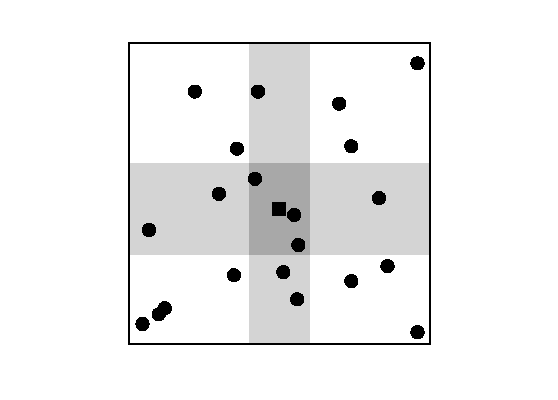
\includegraphics{region.eps}}%
  \end{picture}%
\end{center}
\caption{The calculation of $I_{\text{KL}}(\mathcal{P};h)$. The
  $U$-space corresponds to the horizontal direction, the $V$-space to
  the vertical, of course, this is a cartoon, these spaces are not
  one-dimensional, they do not even have a defined dimension. The
  points in $\mathcal{P}$ are marked as filled circles and a square;
  the square point is the one whose contribution to
  $I_{\text{KL}}(\mathcal{P};h)$ is being calculated. The grey bars
  represent $C_U(\blacksquare)$ and $C_V(\blacksquare)$ with $h=7$,
  that is, each of the grey rectangles contains seven points.
  $\#C(\blacksquare)=4$ since it counts the points in the
  intersection, that is, the region with darker
  shading.\label{fig_region}}
\end{figure}

It is instructive to consider what happens if the two distributions are
independent. In this case the it is possible to calculate the
probability that $\#C(\u_i,\v_i)=r$ for different possible values $r$;
it is a sort of urn problem. 
%
% this makes no sense!
% 2018-08-23
Choosing the $h-1$ points in $C_U(\u_i,\v_i)$ that are not $(\u_i,\v_i)$ itself
is like randomly selecting $h-1$ points out of $n-1$ and calculating $r$ is ask how many
are in $C_V(\u_i,\v_i)$; this gives
%\begin{equation}
%\mbox{prob}\left(\#C(\u_i,\v_i)=r\right)=\frac{\left(\begin{array}{c}h\\r\end{array}\right)
%\left(\begin{array}{c}n-h\\h-r\end{array}\right)}{\left(\begin{array}{c}n\\h\end{array}\right)}
%\end{equation}
\begin{equation}
\mbox{prob}\left(\#C(\u_i,\v_i)=r\right)=\frac{\left(\begin{array}{c}h-1\\r-1\end{array}\right)
\left(\begin{array}{c}n-h\\h-r\end{array}\right)}{\left(\begin{array}{c}n-1\\h-1\end{array}\right)}
\end{equation}
so
\begin{equation}
I_0(n,h)=\sum_{r=1}^h \mbox{prob}\left(\#C(\u_i,\v_i)=r\right) \log_2{\frac{nr}{h^2}}
\end{equation}
is the estimated mutual information when the two distributions are
independent. This is a upward bias in the estimate of the mutual
information; an upward bias is a common feature of estimators of
mutual information. In this case the bias is because $B$ will not
always contain exactly $\langle \#B\rangle$ points. One advantage of
the Kozachenko-Leonenko approach is that $I_0$ gives an explicit
formula for the bias and it depends only on the smoothing parameter
$h$ and the number of pairs, $n$.

Obviously, as $h$ approaches $n$, this bias approaches zero but
otherwise it is positive and as bias it can be removed from the
estimate of the mutual information:
\begin{equation}
I(U;V)\approx\tilde{I}(\mathcal{P};h)=I_{\text{KL}}(\mathcal{P};h)-I_0(n,h)
\end{equation}
Recall that there are two competing approximations used in deriving
the estimate: for small $h$ the counting estimates for the number of
points in a ball and for the volume of the balls are noisy; for large
$h$ the estimate of the probability mass function is too smooth. The
first of these approximations is the cause of the bias described by
$I_0(n,h)$. Conversely $I_0(n,h)$ is not effected by the smoothing
bias. This suggests that the best approximation is found by maximizing
$\tilde{I}(\mathcal{P};h)$ over $h$:
\begin{equation}
I(U;V)\approx\tilde{I}(\mathcal{P})=\max_h{\tilde{I}(\mathcal{P};h)}
\end{equation}
It is demonstrated here that this works very well.

\section{Methods}

\subsection{Data}


\begin{figure}[tp]
\begin{center}
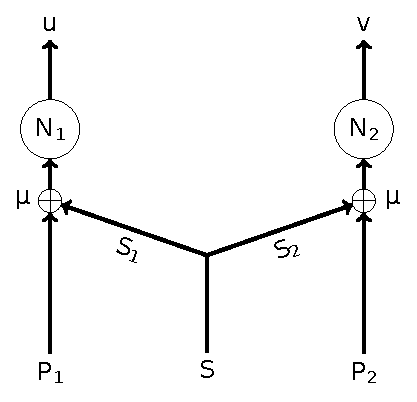
\includegraphics{simulated_data}
\end{center}
\caption{The fictive data. This shows the network used to produce the
  fictive data used to test the density estimation formula for mutual
  information. $N_1$ and $N_2$ are both leaky integrate-and-fire
  neurons, producing the spike trains $\u$ and $\v$
  respectively. Their input is a weighted average of $P_i$ and $S_i$;
  $S$ is a shared input with $S_1=S$ and
  $S_2=\bar{S}-S$.\label{fig_network}}
\end{figure}

The algorithm is run on fictive data generated using two leaky
integrate-and-fire neurons with shared input; the two neurons satisfy
\begin{equation}
\tau_m \frac{dv_i}{dt}=E_l-v_i+I_i
\end{equation}
where, $i=1,2$ labels the two neurons, $\tau_m=12\ms$ and
$E_l=-70\mV$. If $v_i>V_t$, where $V_t=-70\mV$ a spike is recorded and
$v_i$ is reset to $E_l$; there is a refractory period of
$\tau_r=2\ms$. $I_i$ is an input, because the membrane resistance has
been absorbed into $I_i$ it is a voltage rather than a current. Here
\begin{equation}
I_i=(1-\mu) P_i +\mu S_i
\end{equation}
where $P_i$ is an input particular to the $i$ neuron whereas $S_i$ is an
input based on a shared input $S$:
\begin{eqnarray}
S_1&=&S\cr
S_2&=&\bar{S}-S
\end{eqnarray}
with $\bar{S}=30\mV$ and the parameter $\mu$ specifying the amount of
common input.  The inputs $P_i$ and $S$ are both piecewise constant,
with each having a fixed value for a period chosen independently from
a exponential distribution with mean $\tau_c=30\ms$; the value for
each interval is chosen uniformly from $[0,\bar{S}]$. This network is
illustrated in Fig.~\ref{fig_network}.

This method of producing fictive data is not perfect in the sense that
the temporal correlation is different for different values of $\mu$
and the firing rate varies from 32 Hz at $\mu=0$ and $\mu=1$, to 27 Hz
at $\mu=0.5$. However, the aim is to test the spike train pairs with
different values of mutual information and, as will be seen, this
method does succeed in doing that.

\subsection{The distance between spike trains}

For the density estimation information calculation the distance between individual
spike trains is calculated using the van Rossum metric
\citep{vanRossum2001}, this calculates the distance between two spike
trains $\u=(u_1,u_2,\ldots,u_n)$ and
$\v=(v_1,v_2,\ldots,v_m)$ as
\begin{equation}
d(\u,\v)=\sum_{i,j} e^{-|u_i-u_j|/\tau}+\sum_{i,j} e^{-|v_i-v_j|/\tau}-2\sum_{i,j} e^{-|-u_i-v_i|/\tau}
\end{equation}
where $\tau$ is a time scale which can be thought of as expressing the
precision of spike times in neuronal coding. A value around
$\tau=15\ms$ is often used. In the formula for mutual information the
metric is used to order points by proximity so it might be expected
that the values of estimated mutual information would not depend in a
detailed way on the distance values or on the choice of metric. In
fact, it will be seen here that in these data this holds true: the
results are not sensitive to the value of $\tau$.

\subsection{Calculating the information}

The pairs of spike trains produced by the network model are chopped up
into 45 ms intervals. To calculate the mutual information using the
binned method these intervals are discritised with $\delta
t=3\ms$ giving 15 letter words. The frequency for each word pair is
estimated from the data using the obvious empirical estimate
\begin{equation}
p_{U,V}(\u,\v)\approx \frac{\mbox{occurances of }(\u,\v)}{\mbox{total number of samples}}.
\end{equation}
This is then used to calculate the mutual information directly. The
bias is removed by also calculating the mutual information for
shuffled data, in this case this means shuffling the pairing between
the spike train intervals \citep{NirenbergEtAl2001,MontemurroEtAl2007,
  PanzeriEtAl2007,MagriEtAl2009}.

To calculate the mutual information using the density estimation
method, the distance matrix for the $U$-spike trains and the $V$-spike
trains were calculated using the efficient implementation of the van
Rossum metric described in \citep{HoughtonKreuz2012}. The optimal
value of $h$ was found using a golden mean search \citep{Kiefer1953}.

\section{Results}

In Fig.~\ref{fig_mu_sweep} the value of the mutual information for
$45\ms$ intervals of spike train is calculated for different values of
$\mu\in[0,1]$ using both the binned and density estimation approaches. For the density estimation
  approach $200\s$ of data is used; for the binned method
  $25000\s$ of data is used to establish the ground truth and smaller
  value of $2000\s$ to illustrate the amount of data needed to
  estimate the mutual information.

\begin{figure}[tp]

\begin{center}
% GNUPLOT: LaTeX picture with Postscript
\begingroup
  \makeatletter
  \providecommand\color[2][]{%
    \GenericError{(gnuplot) \space\space\space\@spaces}{%
      Package color not loaded in conjunction with
      terminal option `colourtext'%
    }{See the gnuplot documentation for explanation.%
    }{Either use 'blacktext' in gnuplot or load the package
      color.sty in LaTeX.}%
    \renewcommand\color[2][]{}%
  }%
  \providecommand\includegraphics[2][]{%
    \GenericError{(gnuplot) \space\space\space\@spaces}{%
      Package graphicx or graphics not loaded%
    }{See the gnuplot documentation for explanation.%
    }{The gnuplot epslatex terminal needs graphicx.sty or graphics.sty.}%
    \renewcommand\includegraphics[2][]{}%
  }%
  \providecommand\rotatebox[2]{#2}%
  \@ifundefined{ifGPcolor}{%
    \newif\ifGPcolor
    \GPcolorfalse
  }{}%
  \@ifundefined{ifGPblacktext}{%
    \newif\ifGPblacktext
    \GPblacktexttrue
  }{}%
  % define a \g@addto@macro without @ in the name:
  \let\gplgaddtomacro\g@addto@macro
  % define empty templates for all commands taking text:
  \gdef\gplbacktext{}%
  \gdef\gplfronttext{}%
  \makeatother
  \ifGPblacktext
    % no textcolor at all
    \def\colorrgb#1{}%
    \def\colorgray#1{}%
  \else
    % gray or color?
    \ifGPcolor
      \def\colorrgb#1{\color[rgb]{#1}}%
      \def\colorgray#1{\color[gray]{#1}}%
      \expandafter\def\csname LTw\endcsname{\color{white}}%
      \expandafter\def\csname LTb\endcsname{\color{black}}%
      \expandafter\def\csname LTa\endcsname{\color{black}}%
      \expandafter\def\csname LT0\endcsname{\color[rgb]{1,0,0}}%
      \expandafter\def\csname LT1\endcsname{\color[rgb]{0,1,0}}%
      \expandafter\def\csname LT2\endcsname{\color[rgb]{0,0,1}}%
      \expandafter\def\csname LT3\endcsname{\color[rgb]{1,0,1}}%
      \expandafter\def\csname LT4\endcsname{\color[rgb]{0,1,1}}%
      \expandafter\def\csname LT5\endcsname{\color[rgb]{1,1,0}}%
      \expandafter\def\csname LT6\endcsname{\color[rgb]{0,0,0}}%
      \expandafter\def\csname LT7\endcsname{\color[rgb]{1,0.3,0}}%
      \expandafter\def\csname LT8\endcsname{\color[rgb]{0.5,0.5,0.5}}%
    \else
      % gray
      \def\colorrgb#1{\color{black}}%
      \def\colorgray#1{\color[gray]{#1}}%
      \expandafter\def\csname LTw\endcsname{\color{white}}%
      \expandafter\def\csname LTb\endcsname{\color{black}}%
      \expandafter\def\csname LTa\endcsname{\color{black}}%
      \expandafter\def\csname LT0\endcsname{\color{black}}%
      \expandafter\def\csname LT1\endcsname{\color{black}}%
      \expandafter\def\csname LT2\endcsname{\color{black}}%
      \expandafter\def\csname LT3\endcsname{\color{black}}%
      \expandafter\def\csname LT4\endcsname{\color{black}}%
      \expandafter\def\csname LT5\endcsname{\color{black}}%
      \expandafter\def\csname LT6\endcsname{\color{black}}%
      \expandafter\def\csname LT7\endcsname{\color{black}}%
      \expandafter\def\csname LT8\endcsname{\color{black}}%
    \fi
  \fi
  \setlength{\unitlength}{0.0500bp}%
  \begin{picture}(5040.00,3528.00)%
    \gplgaddtomacro\gplbacktext{%
      \csname LTb\endcsname%
      \put(946,901){\makebox(0,0)[r]{\strut{} 0}}%
      \put(946,1295){\makebox(0,0)[r]{\strut{} 0.2}}%
      \put(946,1688){\makebox(0,0)[r]{\strut{} 0.4}}%
      \put(946,2082){\makebox(0,0)[r]{\strut{} 0.6}}%
      \put(946,2476){\makebox(0,0)[r]{\strut{} 0.8}}%
      \put(946,2869){\makebox(0,0)[r]{\strut{} 1}}%
      \put(946,3263){\makebox(0,0)[r]{\strut{} 1.2}}%
      \put(1078,484){\makebox(0,0){\strut{} 0}}%
      \put(1791,484){\makebox(0,0){\strut{} 0.2}}%
      \put(2504,484){\makebox(0,0){\strut{} 0.4}}%
      \put(3217,484){\makebox(0,0){\strut{} 0.6}}%
      \put(3930,484){\makebox(0,0){\strut{} 0.8}}%
      \put(4643,484){\makebox(0,0){\strut{} 1}}%
      \put(176,1983){\rotatebox{-270}{\makebox(0,0){\strut{}mutual information (bits)}}}%
      \put(2860,154){\makebox(0,0){\strut{}$\mu$}}%
    }%
    \gplgaddtomacro\gplfronttext{%
      \csname LTb\endcsname%
      \put(1610,3140){\makebox(0,0)[l]{\strut{}new 200 s}}%
      \csname LTb\endcsname%
      \put(1610,2920){\makebox(0,0)[l]{\strut{}old 2000 s}}%
      \csname LTb\endcsname%
      \put(1610,2700){\makebox(0,0)[l]{\strut{}old 25000 s}}%
    }%
    \gplbacktext
    \put(0,0){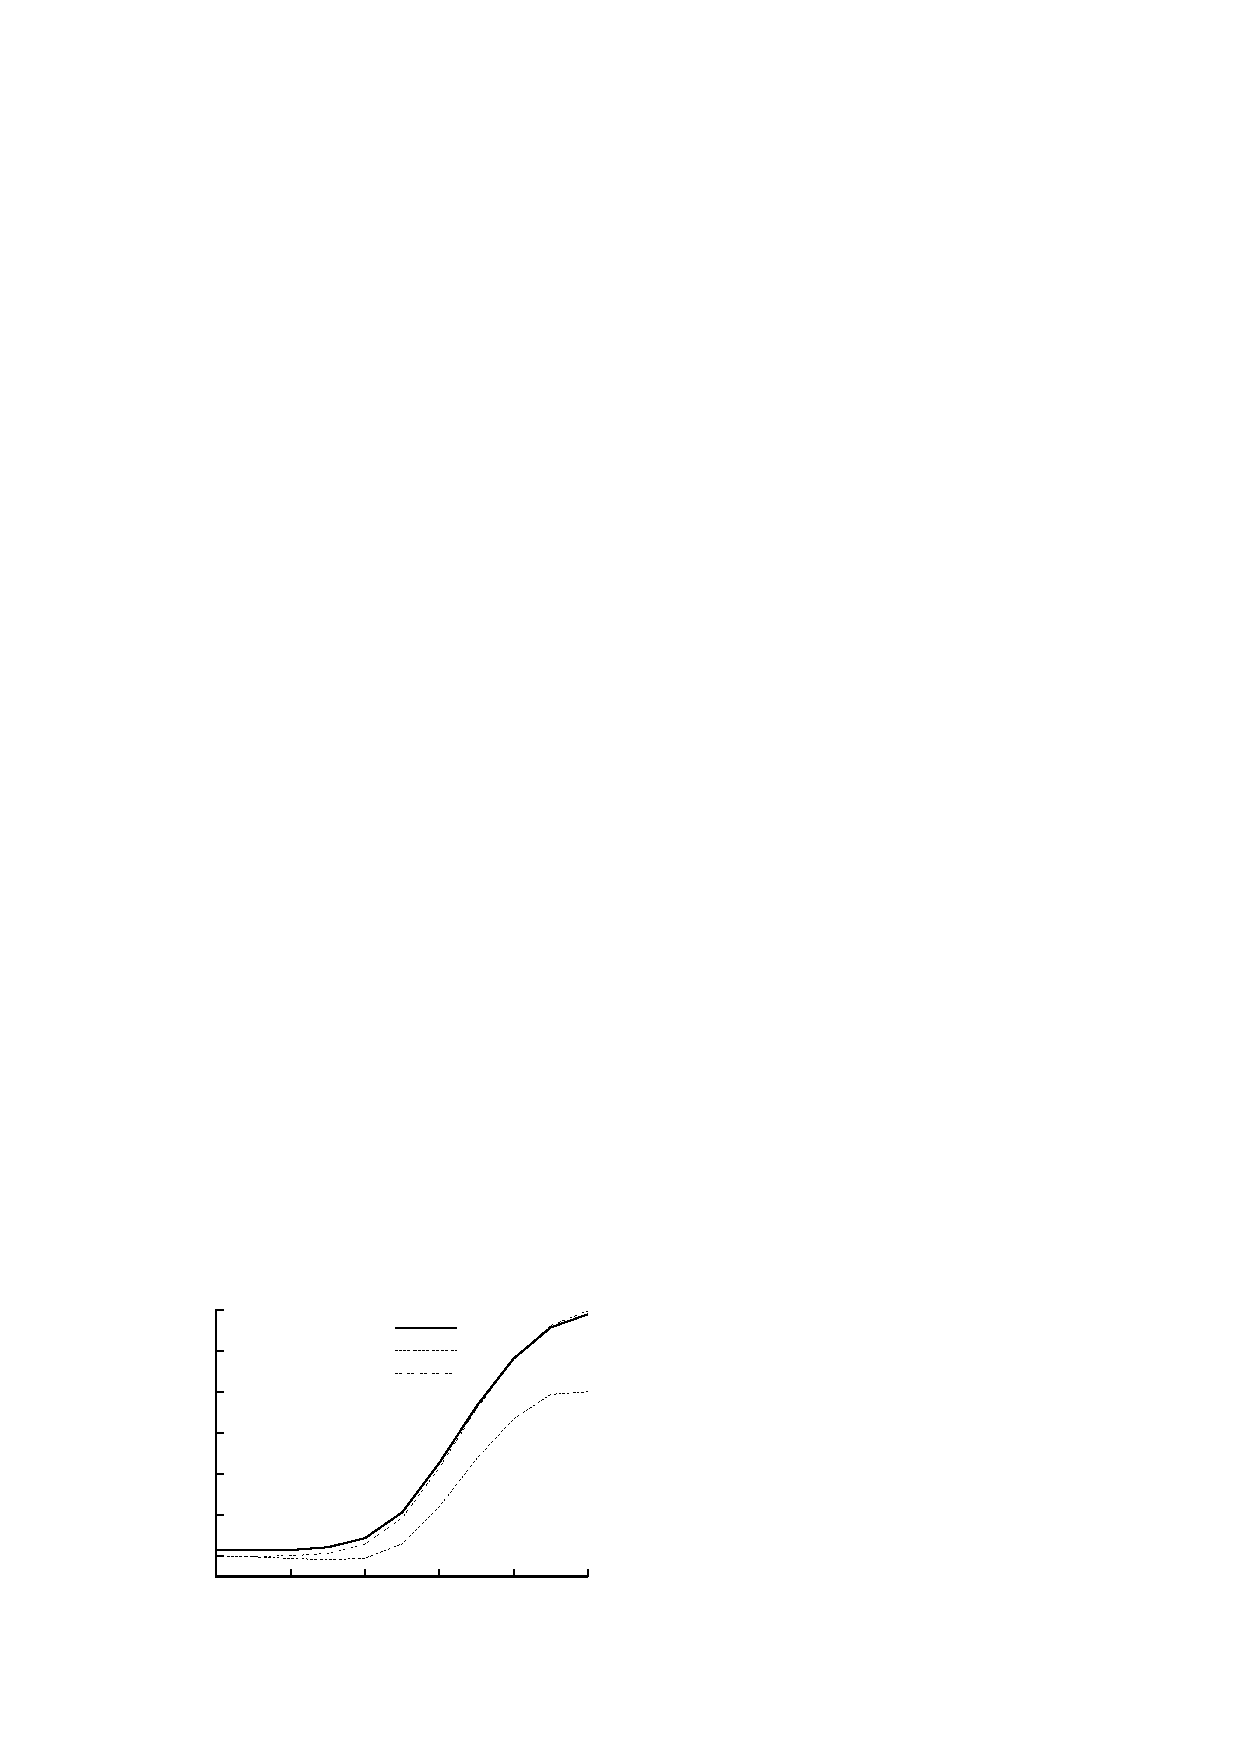
\includegraphics{fig_mu_sweep}}%
    \gplfronttext
  \end{picture}%
\endgroup
\end{center}
\caption{Estimates of the mutual information for different values of
  $\mu$. The mutual information between pairs of 45 ms fragments of
  spike train is estimated using the density estimation, marked
  \lq{}new\rq{} and the binned, marked \lq{}old\rq{}, approaches. In
  the case of the density estimation approach 200 s of spike train is used, in the
  binned approach, 2000 s and 25000 s are used. In all cases the graph
  shows the average of 100 trials; in the density estimation approach $\tau=15\ms$,
  in the binned approach 3 ms bins are used.\label{fig_mu_sweep}}
\end{figure}

Using 2000 s of data the binned method gives a very poor estimate of the
mutual information for most values of $\mu$; the density estimation method is much
closer to the value estimated using 25000 s of data. The binned method
is better for values of $\mu<0.4$ when the amount of mutual
information is very low; presumably this is because the noise in the
estimate is more significant and the maximization over $h$ leads to an
over-estimate.


\begin{figure}[tp]
\begin{center}
% GNUPLOT: LaTeX picture with Postscript
\begingroup
  \makeatletter
  \providecommand\color[2][]{%
    \GenericError{(gnuplot) \space\space\space\@spaces}{%
      Package color not loaded in conjunction with
      terminal option `colourtext'%
    }{See the gnuplot documentation for explanation.%
    }{Either use 'blacktext' in gnuplot or load the package
      color.sty in LaTeX.}%
    \renewcommand\color[2][]{}%
  }%
  \providecommand\includegraphics[2][]{%
    \GenericError{(gnuplot) \space\space\space\@spaces}{%
      Package graphicx or graphics not loaded%
    }{See the gnuplot documentation for explanation.%
    }{The gnuplot epslatex terminal needs graphicx.sty or graphics.sty.}%
    \renewcommand\includegraphics[2][]{}%
  }%
  \providecommand\rotatebox[2]{#2}%
  \@ifundefined{ifGPcolor}{%
    \newif\ifGPcolor
    \GPcolorfalse
  }{}%
  \@ifundefined{ifGPblacktext}{%
    \newif\ifGPblacktext
    \GPblacktexttrue
  }{}%
  % define a \g@addto@macro without @ in the name:
  \let\gplgaddtomacro\g@addto@macro
  % define empty templates for all commands taking text:
  \gdef\gplbacktext{}%
  \gdef\gplfronttext{}%
  \makeatother
  \ifGPblacktext
    % no textcolor at all
    \def\colorrgb#1{}%
    \def\colorgray#1{}%
  \else
    % gray or color?
    \ifGPcolor
      \def\colorrgb#1{\color[rgb]{#1}}%
      \def\colorgray#1{\color[gray]{#1}}%
      \expandafter\def\csname LTw\endcsname{\color{white}}%
      \expandafter\def\csname LTb\endcsname{\color{black}}%
      \expandafter\def\csname LTa\endcsname{\color{black}}%
      \expandafter\def\csname LT0\endcsname{\color[rgb]{1,0,0}}%
      \expandafter\def\csname LT1\endcsname{\color[rgb]{0,1,0}}%
      \expandafter\def\csname LT2\endcsname{\color[rgb]{0,0,1}}%
      \expandafter\def\csname LT3\endcsname{\color[rgb]{1,0,1}}%
      \expandafter\def\csname LT4\endcsname{\color[rgb]{0,1,1}}%
      \expandafter\def\csname LT5\endcsname{\color[rgb]{1,1,0}}%
      \expandafter\def\csname LT6\endcsname{\color[rgb]{0,0,0}}%
      \expandafter\def\csname LT7\endcsname{\color[rgb]{1,0.3,0}}%
      \expandafter\def\csname LT8\endcsname{\color[rgb]{0.5,0.5,0.5}}%
    \else
      % gray
      \def\colorrgb#1{\color{black}}%
      \def\colorgray#1{\color[gray]{#1}}%
      \expandafter\def\csname LTw\endcsname{\color{white}}%
      \expandafter\def\csname LTb\endcsname{\color{black}}%
      \expandafter\def\csname LTa\endcsname{\color{black}}%
      \expandafter\def\csname LT0\endcsname{\color{black}}%
      \expandafter\def\csname LT1\endcsname{\color{black}}%
      \expandafter\def\csname LT2\endcsname{\color{black}}%
      \expandafter\def\csname LT3\endcsname{\color{black}}%
      \expandafter\def\csname LT4\endcsname{\color{black}}%
      \expandafter\def\csname LT5\endcsname{\color{black}}%
      \expandafter\def\csname LT6\endcsname{\color{black}}%
      \expandafter\def\csname LT7\endcsname{\color{black}}%
      \expandafter\def\csname LT8\endcsname{\color{black}}%
    \fi
  \fi
  \setlength{\unitlength}{0.0500bp}%
  \begin{picture}(7300.00,5520.00)%
      \put(846,5700){\makebox(0,0)[r]{\strut{} \textbf{A}}}%
      \put(946,3704){\makebox(0,0)[r]{\strut{} 0}}%
      \put(946,4092){\makebox(0,0)[r]{\strut{} 0.2}}%
      \put(946,4480){\makebox(0,0)[r]{\strut{} 0.4}}%
      \put(946,4868){\makebox(0,0)[r]{\strut{} 0.6}}%
      \put(946,5256){\makebox(0,0)[r]{\strut{} 0.8}}%
      \put(1589,3484){\makebox(0,0){\strut{} 100}}%
      \put(2127,3484){\makebox(0,0){\strut{} 200}}%
      \put(2665,3484){\makebox(0,0){\strut{} 300}}%
      \put(3203,3484){\makebox(0,0){\strut{} 400}}%
      \put(176,4480){\rotatebox{-270}{\makebox(0,0){\strut{}mutual information (bits)}}}%
      \put(3876,4480){\rotatebox{-270}{\makebox(0,0){\strut{}mutual information (bits)}}}%
      \put(2140,3154){\makebox(0,0){\strut{}spike train length (s)}}%

      \put(4546,5700){\makebox(0,0)[r]{\strut{} \textbf{B}}}%
      \put(4646,3704){\makebox(0,0)[r]{\strut{}-0.2}}%
      \put(4646,4014){\makebox(0,0)[r]{\strut{} 0}}%
      \put(4646,4325){\makebox(0,0)[r]{\strut{} 0.2}}%
      \put(4646,4635){\makebox(0,0)[r]{\strut{} 0.4}}%
      \put(4646,4946){\makebox(0,0)[r]{\strut{} 0.6}}%
      \put(4646,5256){\makebox(0,0)[r]{\strut{} 0.8}}%
      \put(5836,3484){\makebox(0,0){\strut{} 12500}}%
      \put(6903,3484){\makebox(0,0){\strut{} 25000}}%
      \put(5840,3154){\makebox(0,0){\strut{}spike train length (s)}}%


      \put(846,2700){\makebox(0,0)[r]{\strut{} \textbf{C}}}%

      \put(946,704){\makebox(0,0)[r]{\strut{}-0.2}}%
      \put(946,1014){\makebox(0,0)[r]{\strut{} 0}}%
      \put(946,1325){\makebox(0,0)[r]{\strut{} 0.2}}%
      \put(946,1635){\makebox(0,0)[r]{\strut{} 0.4}}%
      \put(946,1946){\makebox(0,0)[r]{\strut{} 0.6}}%
      \put(946,2256){\makebox(0,0)[r]{\strut{} 0.8}}%
      \put(1251,484){\makebox(0,0){\strut{} 1}}%
      \put(1825,484){\makebox(0,0){\strut{} 2}}%
      \put(2400,484){\makebox(0,0){\strut{} 3}}%
      \put(2974,484){\makebox(0,0){\strut{} 4}}%
      \put(176,1480){\rotatebox{-270}{\makebox(0,0){\strut{}mutual information (bits)}}}%
      \put(2140,154){\makebox(0,0){\strut{}$\log_{10}($spike train length$)$}}%

      \put(2216,1097){\makebox(0,0)[r]{\strut{}new}}%
      \put(2216,877){\makebox(0,0)[r]{\strut{}old}}%

      \put(4546,2700){\makebox(0,0)[r]{\strut{} \textbf{D}}}%
      \put(4778,705){\makebox(0,0)[r]{\strut{} 0}}%
      \put(4778,1093){\makebox(0,0)[r]{\strut{} 0.03}}%
      \put(4778,1481){\makebox(0,0)[r]{\strut{} 0.06}}%
      \put(4778,1868){\makebox(0,0)[r]{\strut{} 0.09}}%
      \put(4778,2256){\makebox(0,0)[r]{\strut{} 0.12}}%
      \put(5389,484){\makebox(0,0){\strut{} 100}}%
      \put(5894,484){\makebox(0,0){\strut{} 200}}%
      \put(6398,484){\makebox(0,0){\strut{} 300}}%
      \put(6903,484){\makebox(0,0){\strut{} 400}}%
      \put(3876,1480){\rotatebox{-270}{\makebox(0,0){\strut{}standard deviation (bits)}}}%
      \put(5906,154){\makebox(0,0){\strut{}spike train length (s)}}%
      \put(5916,2083){\makebox(0,0)[r]{\strut{}new}}%
      \put(5916,1863){\makebox(0,0)[r]{\strut{}old}}%


    \put(0,3000){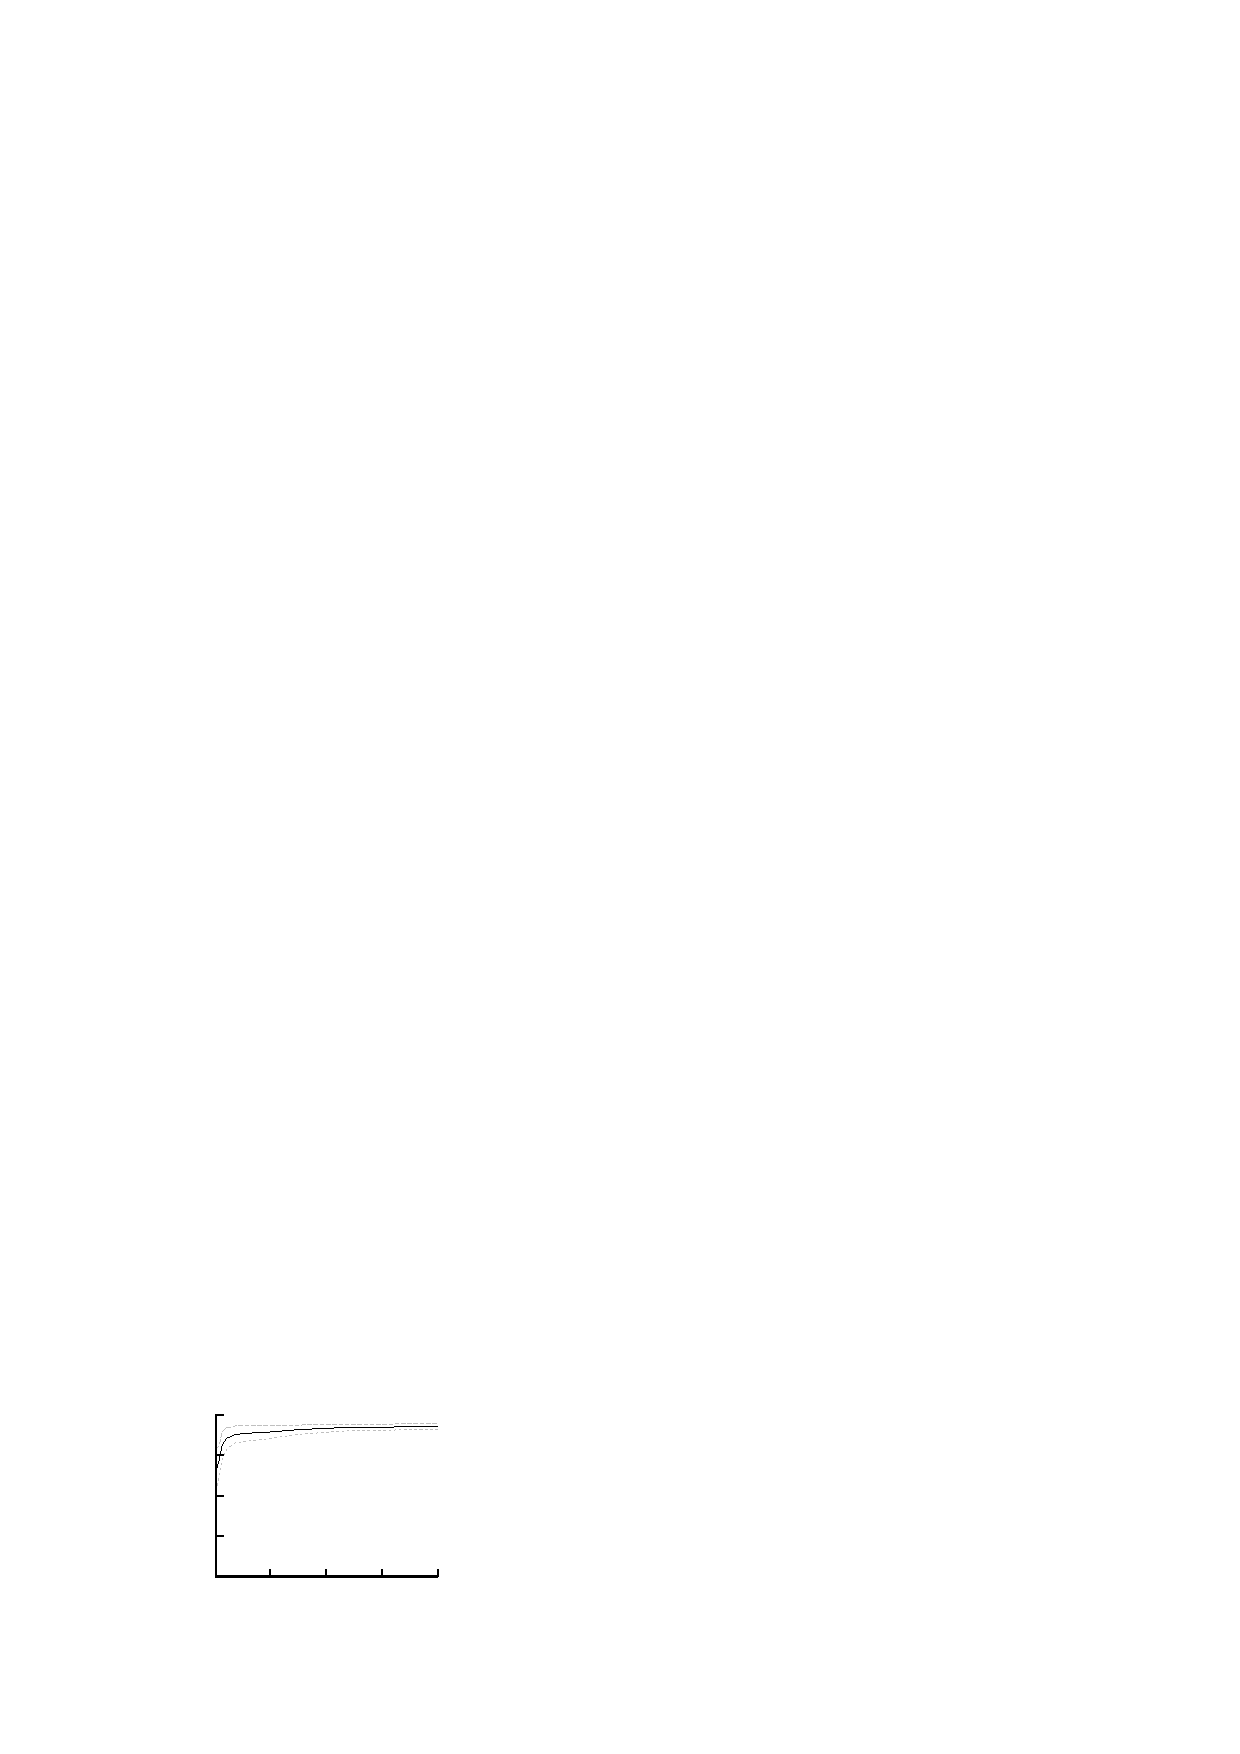
\includegraphics{length_sweep_new}}
    \put(3700,3000){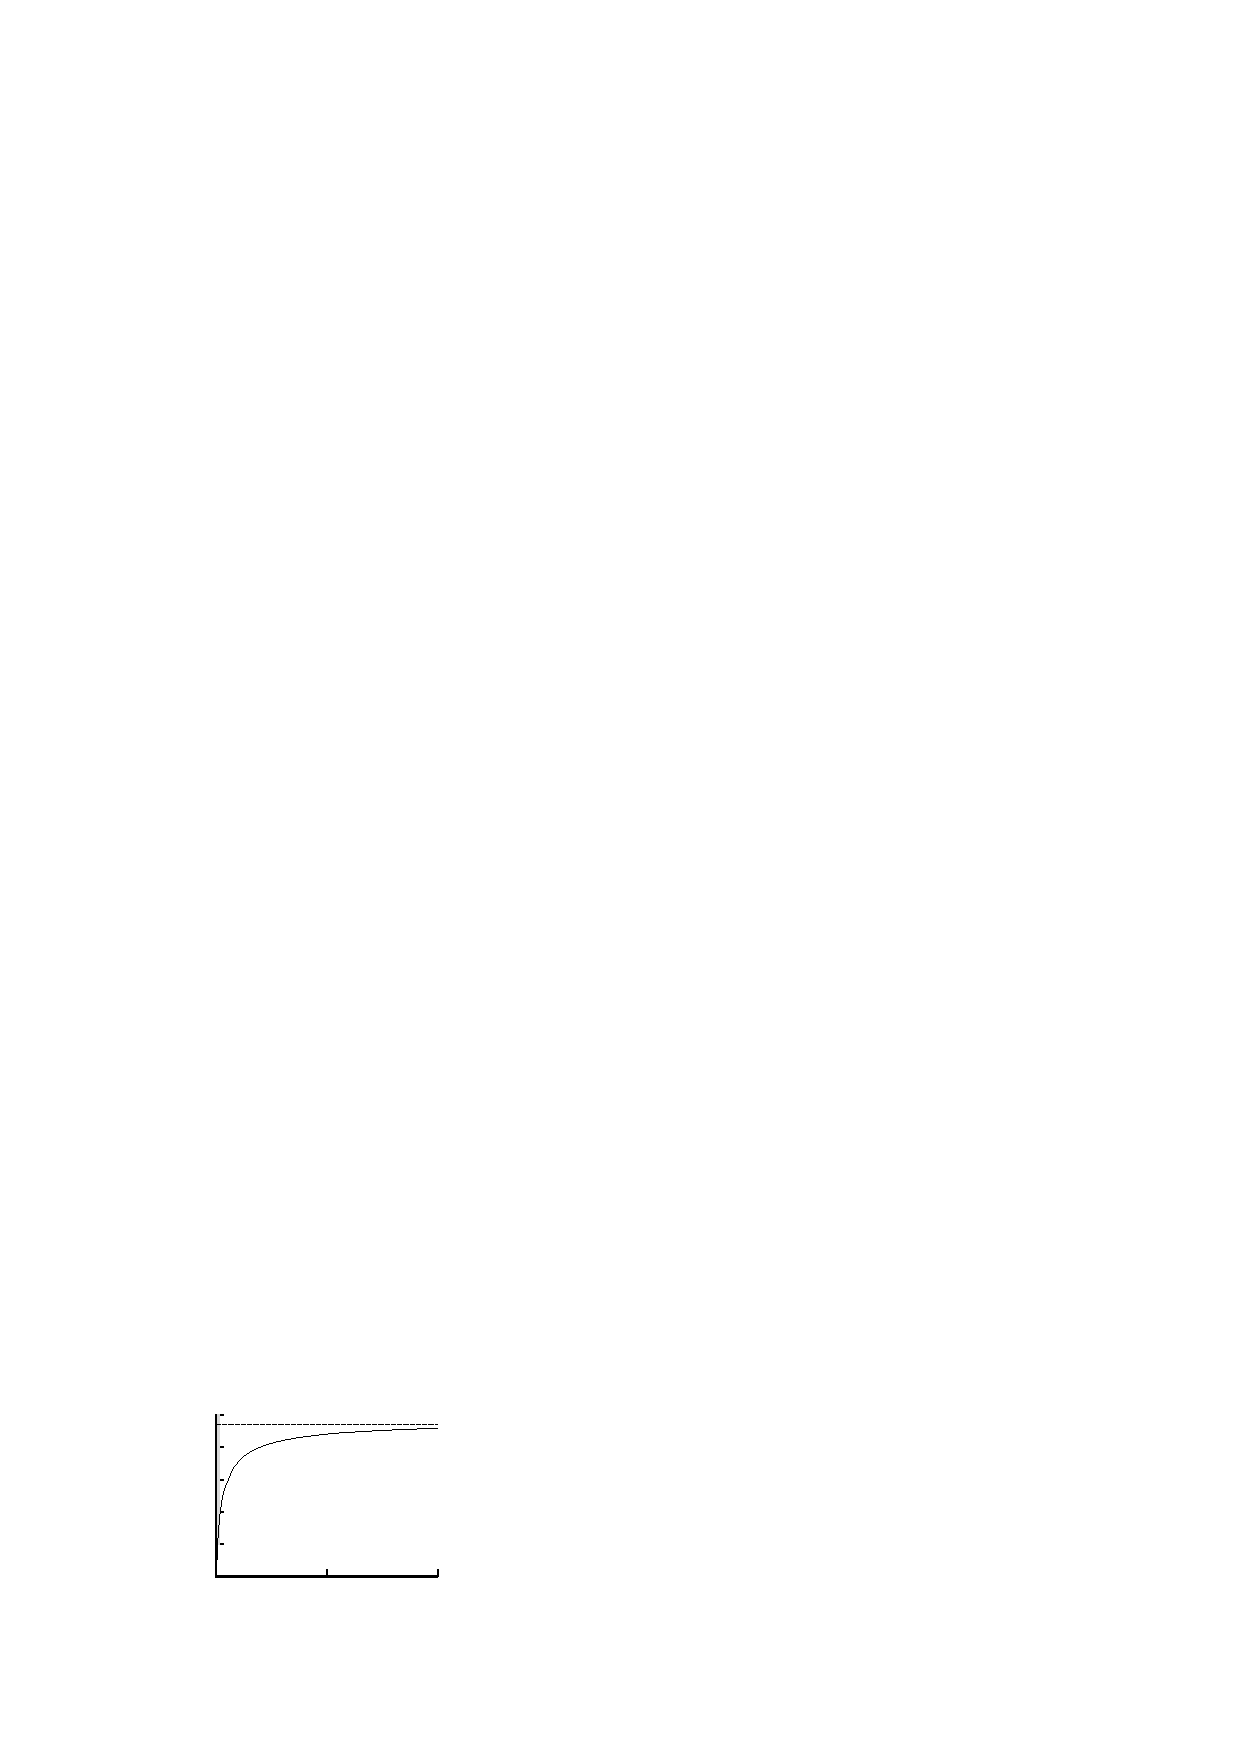
\includegraphics{length_sweep_old}}%
    \put(3700,0){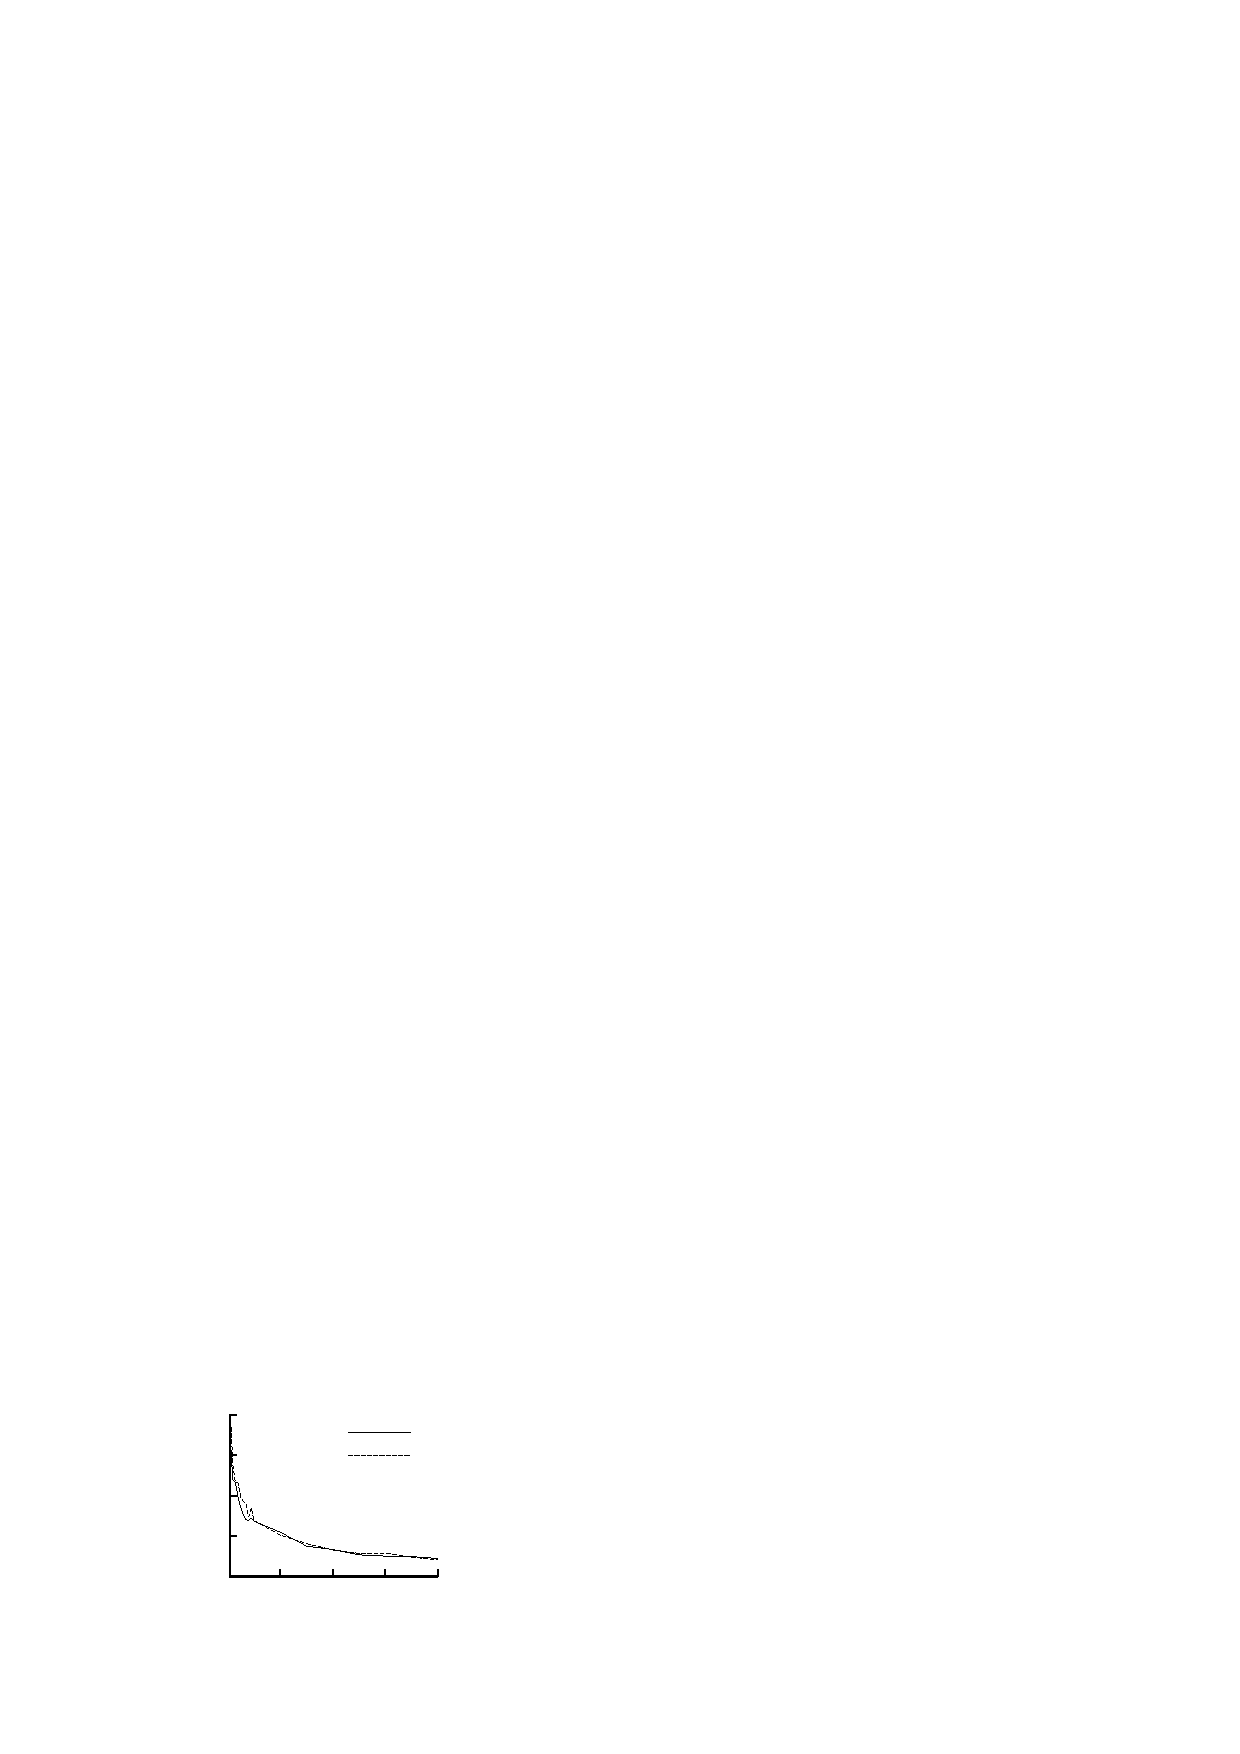
\includegraphics{fig_sd}}%
    \put(0,0){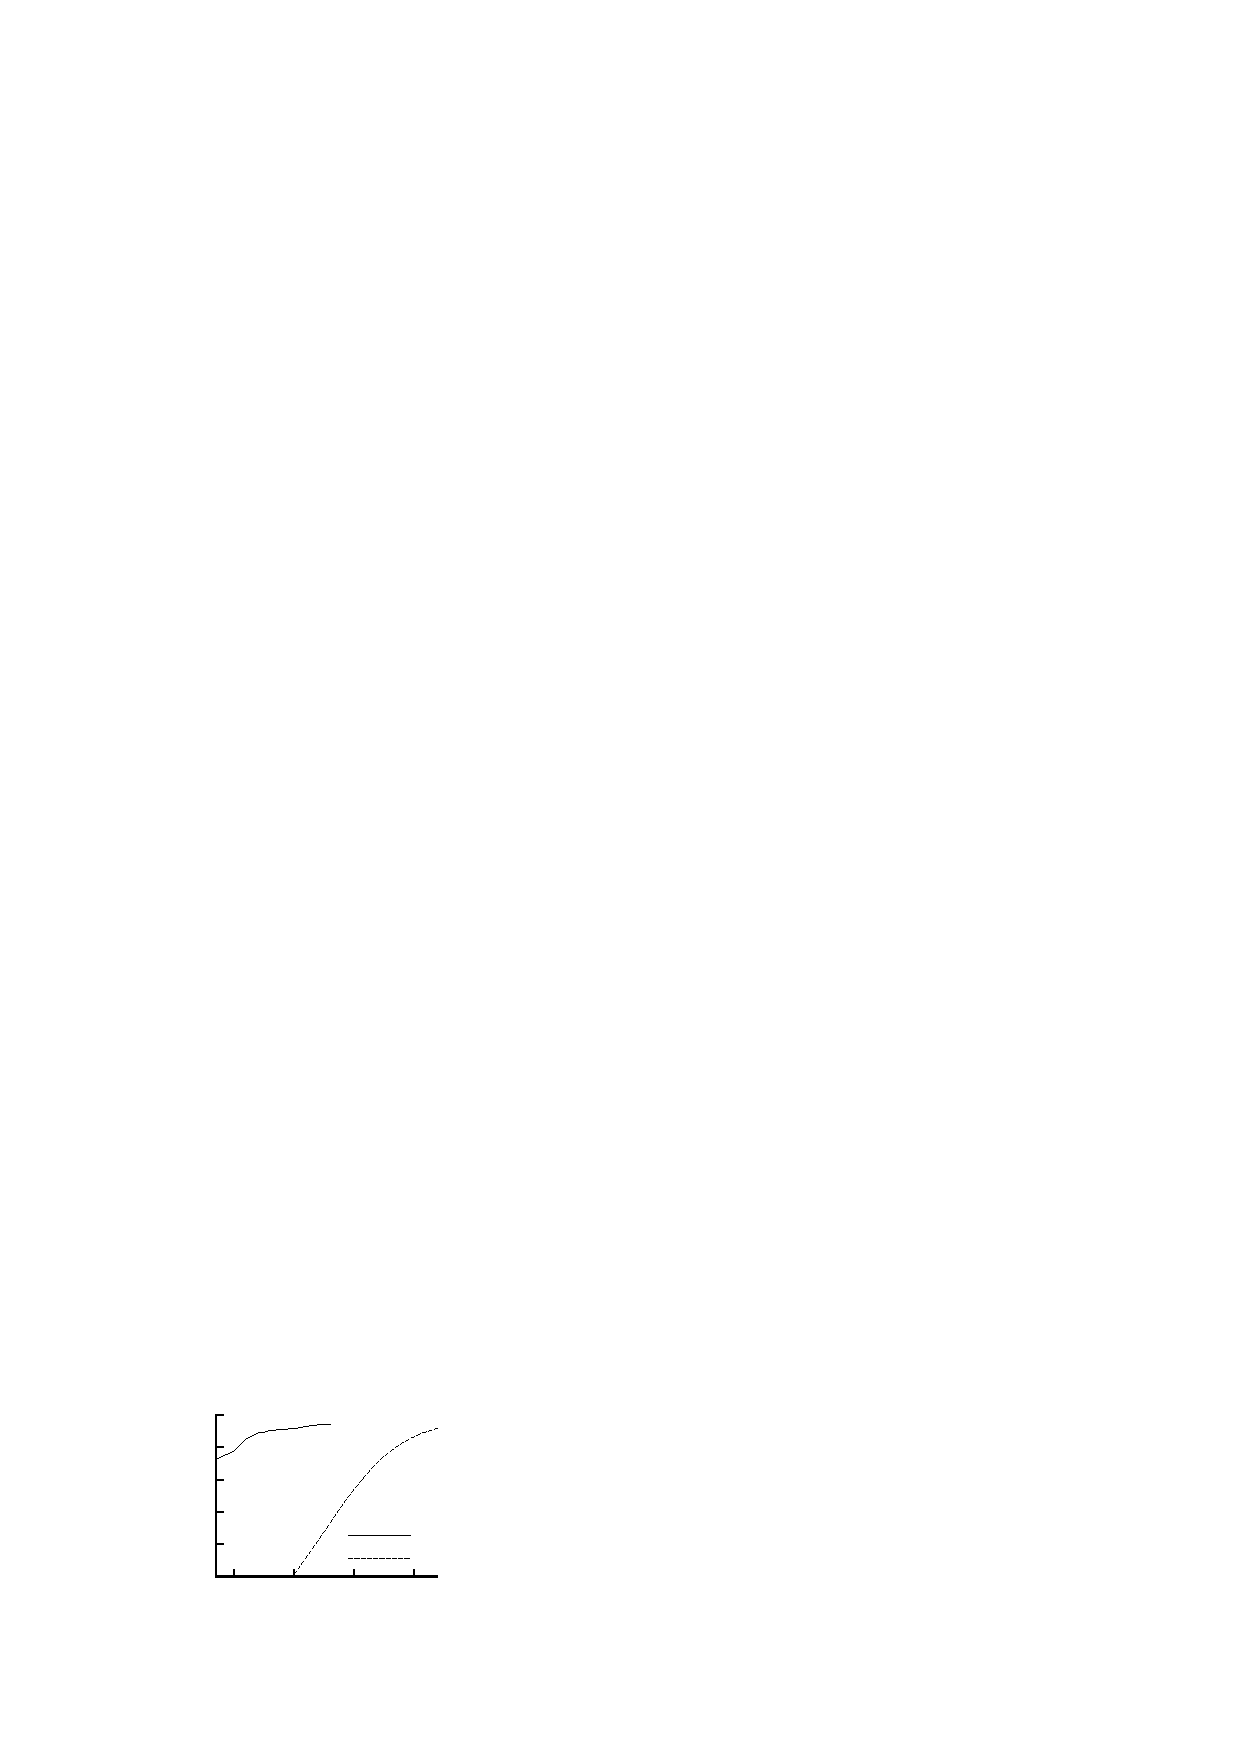
\includegraphics{fig_length_sweep_log}}%
  \end{picture}%
\endgroup
\end{center}
\caption{Performance of the formula for calculating mutual
  information. All these graphs concern pairs of spike trains where
  $\mu=0.7$ and the mutual information is being calculated between 45
  ms fragments. \textbf{A} and \textbf{B} compare the density
  estimation (\textbf{A}) and binned (\textbf{B}) approaches to
  calculating mutual information as longer and longer spike trains are
  used. In \textbf{B} the very thin grey rectangle along the vertical
  axis marks out the area shown in \textbf{A} and the horizontal line
  gives the value estimated by the density estimation approach using
  400 s spike trains. These two graphs are shown again in \textbf{C}
  where a log-scale is used for spike train length. In both \textbf{A}
  and \textbf{B} the plots are of the mean over 100 trials, in
  \textbf{A} the dotted lines show one standard deviation from the
  mean. For \textbf{B} the standard deviation is vanishingly
  small, this is because so much data is used in this approach. In \textbf{D} the
  standard deviation using the density estimation and binned
  approaches are compared, they are roughly similar, though, of
  course, in the binned approach the mean is very different from the
  value estimated using more data.
 \label{fig_length_sweep}}
\end{figure}


Fig.~\ref{fig_length_sweep}\textbf{A} and \textbf{B} show the
convergence of the density estimation and binned methods;
Fig.~\ref{fig_length_sweep}\textbf{C} uses a log scale to exhibit both
on the same graph. These graphs show that the density estimation
method uses considerably less data than the binned method. It is clear
from these graphs that the estimators approach their asymptotic values
in an orderly way. This means one approach, described in
\cite{TrevesPanzeri1995,StrongEtAl1998,PanzeriEtAl2007}, to improving
the estimate using the binned method is to fit the graph to a curve
such as
\begin{equation}
I(a,b,c)=a+\frac{b}{\sqrt{T}}+\frac{c}{T\sqrt{T}}
\end{equation}
where $T$ is the length of spike train used. For the simulated data
being examined here this works quite well, concentrating on $\mu=0.7$
as an example, fixing $a$, $b$ and $c$ using the first $2000$ s, gives
an estimate of $0.6613$ for $T=25000\s$, compared to an actual value
of $0.7156$; the value given by the density estimation method using
400 s of data is $0.7412$. The binned method gives even larger values
if even larger amounts of data are used, for this value of $\mu$
1000000 s of data gives 0.768413. Extrapolating the binned method from
200 s of data does not work, it gives an estimate of
$0.1975$. Fig.~\ref{fig_length_sweep}\textbf{D} compares the standard
deviation for the two methods; they are roughly the same. 


\begin{figure}[tp]
\begin{center}
% GNUPLOT: LaTeX picture with Postscript
\begingroup
  \makeatletter
  \providecommand\color[2][]{%
    \GenericError{(gnuplot) \space\space\space\@spaces}{%
      Package color not loaded in conjunction with
      terminal option `colourtext'%
    }{See the gnuplot documentation for explanation.%
    }{Either use 'blacktext' in gnuplot or load the package
      color.sty in LaTeX.}%
    \renewcommand\color[2][]{}%
  }%
  \providecommand\includegraphics[2][]{%
    \GenericError{(gnuplot) \space\space\space\@spaces}{%
      Package graphicx or graphics not loaded%
    }{See the gnuplot documentation for explanation.%
    }{The gnuplot epslatex terminal needs graphicx.sty or graphics.sty.}%
    \renewcommand\includegraphics[2][]{}%
  }%
  \providecommand\rotatebox[2]{#2}%
  \@ifundefined{ifGPcolor}{%
    \newif\ifGPcolor
    \GPcolorfalse
  }{}%
  \@ifundefined{ifGPblacktext}{%
    \newif\ifGPblacktext
    \GPblacktexttrue
  }{}%
  % define a \g@addto@macro without @ in the name:
  \let\gplgaddtomacro\g@addto@macro
  % define empty templates for all commands taking text:
  \gdef\gplbacktext{}%
  \gdef\gplfronttext{}%
  \makeatother
  \ifGPblacktext
    % no textcolor at all
    \def\colorrgb#1{}%
    \def\colorgray#1{}%
  \else
    % gray or color?
    \ifGPcolor
      \def\colorrgb#1{\color[rgb]{#1}}%
      \def\colorgray#1{\color[gray]{#1}}%
      \expandafter\def\csname LTw\endcsname{\color{white}}%
      \expandafter\def\csname LTb\endcsname{\color{black}}%
      \expandafter\def\csname LTa\endcsname{\color{black}}%
      \expandafter\def\csname LT0\endcsname{\color[rgb]{1,0,0}}%
      \expandafter\def\csname LT1\endcsname{\color[rgb]{0,1,0}}%
      \expandafter\def\csname LT2\endcsname{\color[rgb]{0,0,1}}%
      \expandafter\def\csname LT3\endcsname{\color[rgb]{1,0,1}}%
      \expandafter\def\csname LT4\endcsname{\color[rgb]{0,1,1}}%
      \expandafter\def\csname LT5\endcsname{\color[rgb]{1,1,0}}%
      \expandafter\def\csname LT6\endcsname{\color[rgb]{0,0,0}}%
      \expandafter\def\csname LT7\endcsname{\color[rgb]{1,0.3,0}}%
      \expandafter\def\csname LT8\endcsname{\color[rgb]{0.5,0.5,0.5}}%
    \else
      % gray
      \def\colorrgb#1{\color{black}}%
      \def\colorgray#1{\color[gray]{#1}}%
      \expandafter\def\csname LTw\endcsname{\color{white}}%
      \expandafter\def\csname LTb\endcsname{\color{black}}%
      \expandafter\def\csname LTa\endcsname{\color{black}}%
      \expandafter\def\csname LT0\endcsname{\color{black}}%
      \expandafter\def\csname LT1\endcsname{\color{black}}%
      \expandafter\def\csname LT2\endcsname{\color{black}}%
      \expandafter\def\csname LT3\endcsname{\color{black}}%
      \expandafter\def\csname LT4\endcsname{\color{black}}%
      \expandafter\def\csname LT5\endcsname{\color{black}}%
      \expandafter\def\csname LT6\endcsname{\color{black}}%
      \expandafter\def\csname LT7\endcsname{\color{black}}%
      \expandafter\def\csname LT8\endcsname{\color{black}}%
    \fi
  \fi
  \setlength{\unitlength}{0.0500bp}%
  \begin{picture}(7300.00,5520.00)%
      \put(846,5700){\makebox(0,0)[r]{\strut{} \textbf{A}}}%

      \put(1078,3845){\makebox(0,0)[r]{\strut{} 0}}%
      \put(1078,4198){\makebox(0,0)[r]{\strut{} 0.25}}%
      \put(1078,4551){\makebox(0,0)[r]{\strut{} 0.5}}%
      \put(1078,4903){\makebox(0,0)[r]{\strut{} 0.75}}%
      \put(1078,5256){\makebox(0,0)[r]{\strut{} 1}}%
      \put(1210,3484){\makebox(0,0){\strut{} 0}}%
      \put(1609,3484){\makebox(0,0){\strut{} 0.2}}%
      \put(2007,3484){\makebox(0,0){\strut{} 0.4}}%
      \put(2406,3484){\makebox(0,0){\strut{} 0.6}}%
      \put(2804,3484){\makebox(0,0){\strut{} 0.8}}%
      \put(3203,3484){\makebox(0,0){\strut{} 1}}%
      \put(176,4480){\rotatebox{-270}{\makebox(0,0){\strut{}mutual information (bits)}}}%
      \put(2206,3154){\makebox(0,0){\strut{}$\mu$}}%
      \put(1342,5083){\makebox(0,0)[l]{\strut{}new}}%
      \put(1342,4863){\makebox(0,0)[l]{\strut{}old 3 ms}}%
      \put(1342,4643){\makebox(0,0)[l]{\strut{}old 2 ms}}%

      \put(4546,5700){\makebox(0,0)[r]{\strut{} \textbf{B}}}%

      \put(4646,3801){\makebox(0,0)[r]{\strut{} 0}}%
      \put(4646,4286){\makebox(0,0)[r]{\strut{} 0.5}}%
      \put(4646,4771){\makebox(0,0)[r]{\strut{} 1}}%
      \put(4646,5256){\makebox(0,0)[r]{\strut{} 1.5}}%
      \put(4778,3484){\makebox(0,0){\strut{} 0}}%
      \put(5203,3484){\makebox(0,0){\strut{} 0.2}}%
      \put(5628,3484){\makebox(0,0){\strut{} 0.4}}%
      \put(6053,3484){\makebox(0,0){\strut{} 0.6}}%
      \put(6478,3484){\makebox(0,0){\strut{} 0.8}}%
      \put(6903,3484){\makebox(0,0){\strut{} 1}}%
      \put(3876,4480){\rotatebox{-270}{\makebox(0,0){\strut{}mutual information (bits)}}}%
      \put(5840,3154){\makebox(0,0){\strut{}$\mu$}}%
      \put(4910,5083){\makebox(0,0)[l]{\strut{}new}}%
      \put(4910,4863){\makebox(0,0)[l]{\strut{}old}}%



      \put(846,2700){\makebox(0,0)[r]{\strut{} \textbf{C}}}%

      \put(682,738){\makebox(0,0)[r]{\strut{} 0}}%
      \put(682,1075){\makebox(0,0)[r]{\strut{} 1}}%
      \put(682,1413){\makebox(0,0)[r]{\strut{} 2}}%
      \put(682,1750){\makebox(0,0)[r]{\strut{} 3}}%
      \put(682,2087){\makebox(0,0)[r]{\strut{} 4}}%
      \put(814,484){\makebox(0,0){\strut{} 0}}%
      \put(1292,484){\makebox(0,0){\strut{} 0.2}}%
      \put(1770,484){\makebox(0,0){\strut{} 0.4}}%
      \put(2247,484){\makebox(0,0){\strut{} 0.6}}%
      \put(2725,484){\makebox(0,0){\strut{} 0.8}}%
      \put(3203,484){\makebox(0,0){\strut{} 1}}%
      \put(176,1480){\rotatebox{-270}{\makebox(0,0){\strut{}mutual information (bits)}}}%
      \put(2008,154){\makebox(0,0){\strut{}$\mu$}}%

      \put(946,2083){\makebox(0,0)[l]{\strut{}new}}%
      \put(946,1863){\makebox(0,0)[l]{\strut{}old}}%

      \put(4546,2700){\makebox(0,0)[r]{\strut{} \textbf{D}}}%

      \put(4646,778){\makebox(0,0)[r]{\strut{} 0}}%
      \put(4646,1147){\makebox(0,0)[r]{\strut{} 0.5}}%
      \put(4646,1517){\makebox(0,0)[r]{\strut{} 1}}%
      \put(4646,1886){\makebox(0,0)[r]{\strut{} 1.5}}%
      \put(4646,2256){\makebox(0,0)[r]{\strut{} 2}}%
      \put(4778,484){\makebox(0,0){\strut{} 0}}%
      \put(5203,484){\makebox(0,0){\strut{} 0.2}}%
      \put(5628,484){\makebox(0,0){\strut{} 0.4}}%
      \put(6053,484){\makebox(0,0){\strut{} 0.6}}%
      \put(6478,484){\makebox(0,0){\strut{} 0.8}}%
      \put(6903,484){\makebox(0,0){\strut{} 1}}%
      \put(3876,1480){\rotatebox{-270}{\makebox(0,0){\strut{}mutual information (bits)}}}%
      \put(5840,154){\makebox(0,0){\strut{}$\mu$}}%
      \put(4910,2083){\makebox(0,0)[l]{\strut{}new}}%
      \put(4910,1863){\makebox(0,0)[l]{\strut{}old}}%


    \put(0,3000){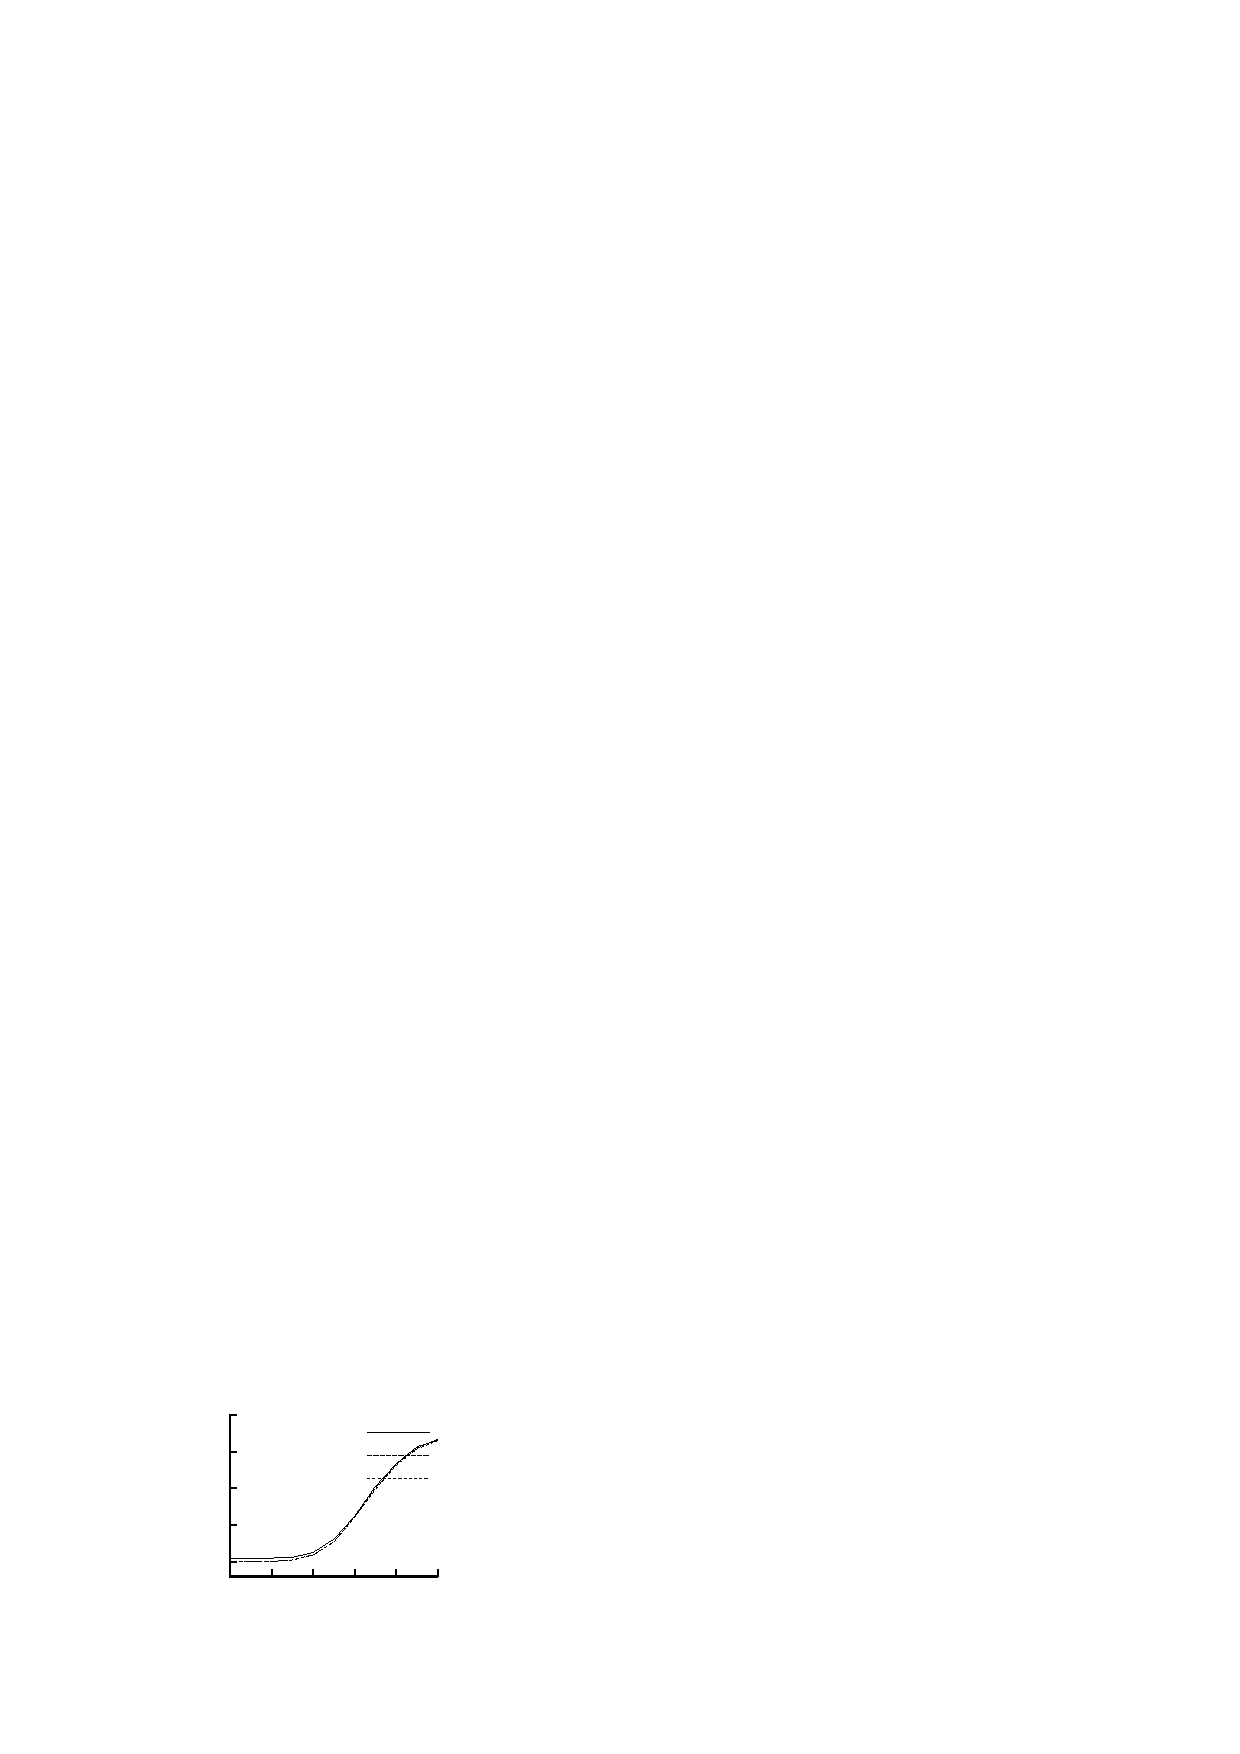
\includegraphics{fig_short_window}}
    \put(3700,3000){
\includegraphics{fig_long_window}}%
    \put(3700,0){
\includegraphics{fig_high_rate}}%
    \put(0,0){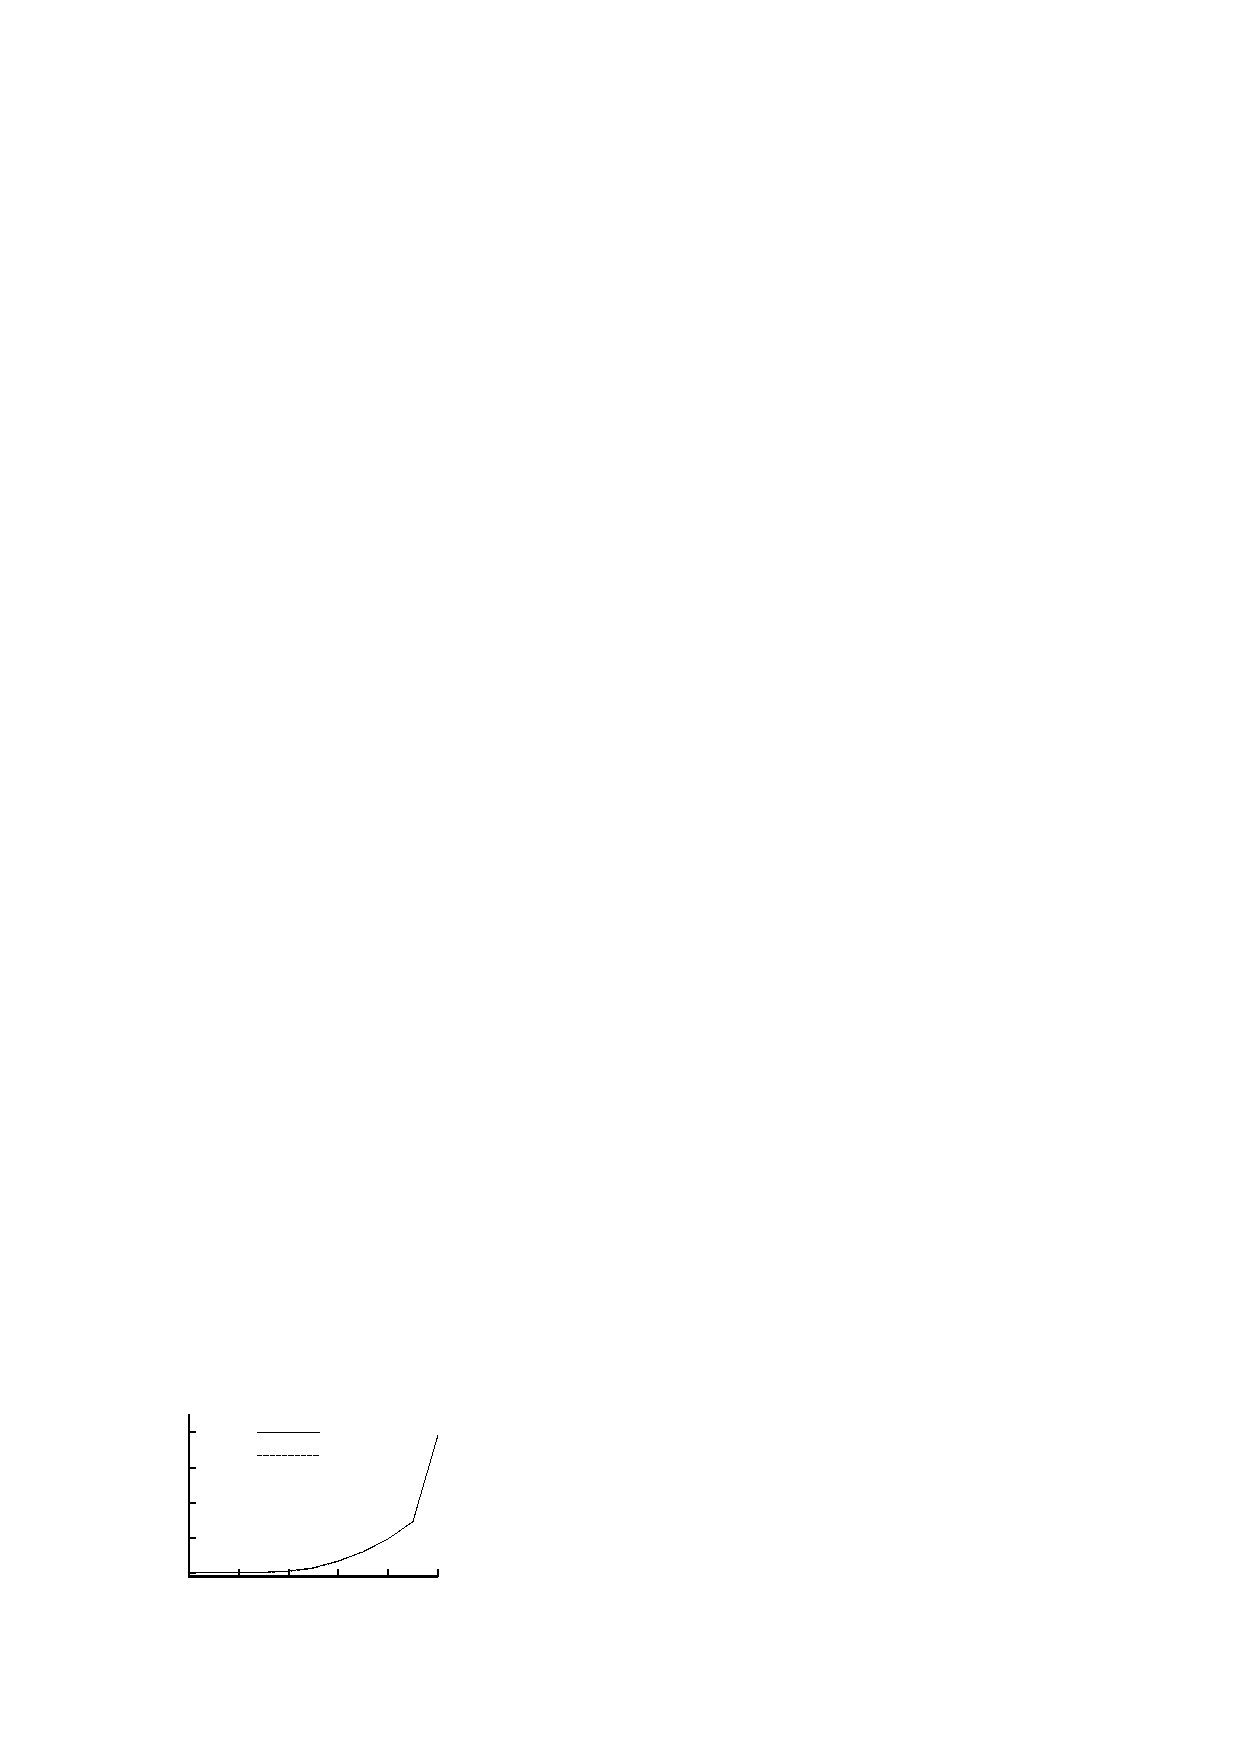
\includegraphics{fig_new_noise}}%


  \end{picture}%
\endgroup
\end{center}
\caption{Testing the robustness of the density estimation approach. In
  \textbf{A} and \textbf{B} the length of the spike train intervals is
  changed. In \textbf{A} they are shortened to 30 ms, in \textbf{B}
  they are increased to 60 ms. In each case for the binned approach,
  marked \lq{}old\rq{}, the intervals are discretized into 3 ms
  letters, in \textbf{A}, the binned approach with 2 ms letters is
  also plotted. In \textbf{C} an alternative model is used to produce
  the simulated data: the shared input is the same, so the input is
  $S_i=S$ for both values of $i$. In \textbf{D} $\bar{S}=35\mV$ is
  used to generate the simulated data, this increases the firing rate
  so that it varies from 44 Hz at $\mu=0$ and $\mu=1$ to 39 Hz at
  $\mu=0.5$. For the binned approach, 25000 s of spike trains are used
  in used in each case.  For the density estimation approach, marked
  \lq{}new\rq{}, 200 s of spike trains are used in \textbf{A} and
  \textbf{C} and 500 s in \textbf{B} and \textbf{D}; when the
  intervals contain on average more spikes the density estimation
  approach appears to require more data. In \textbf{D} the difference
  between the two approaches is more noticeable for $\mu$ near one
  than in other graphs. \label{fig_different_mu_sweeps}}
\end{figure}



The robustness of the density estimation approach to mutual
information is examined in Fig.~\ref{fig_different_mu_sweeps}. In
Fig.~\ref{fig_different_mu_sweeps}\textbf{A} and
Fig.~\ref{fig_different_mu_sweeps}\textbf{B} the lengths of the short intervals
used to calculate the mutual information are changed;
Fig.~\ref{fig_different_mu_sweeps}\textbf{A} also plots the binned
estimate with a different letter length. In
Fig.~\ref{fig_different_mu_sweeps}\textbf{C} a different stimulus is
used, whereas for all the other simulations the
shared input is shared with $S_1=S$ and $S_2=\bar{S}-S$, in this
figure $S_i=S$ for both values of $i$. Finally, in
Fig.~\ref{fig_different_mu_sweeps}\textbf{D} an input with a higher
firing rate is used. The density estimator performs well, but there is
some indication that the amount of data required, though modest
compared to the binned approach, does increase as the number of spikes
increases.


\begin{figure}[tp]
\begin{center}
% GNUPLOT: LaTeX picture with Postscript
\begingroup
  \makeatletter
  \providecommand\color[2][]{%
    \GenericError{(gnuplot) \space\space\space\@spaces}{%
      Package color not loaded in conjunction with
      terminal option `colourtext'%
    }{See the gnuplot documentation for explanation.%
    }{Either use 'blacktext' in gnuplot or load the package
      color.sty in LaTeX.}%
    \renewcommand\color[2][]{}%
  }%
  \providecommand\includegraphics[2][]{%
    \GenericError{(gnuplot) \space\space\space\@spaces}{%
      Package graphicx or graphics not loaded%
    }{See the gnuplot documentation for explanation.%
    }{The gnuplot epslatex terminal needs graphicx.sty or graphics.sty.}%
    \renewcommand\includegraphics[2][]{}%
  }%
  \providecommand\rotatebox[2]{#2}%
  \@ifundefined{ifGPcolor}{%
    \newif\ifGPcolor
    \GPcolorfalse
  }{}%
  \@ifundefined{ifGPblacktext}{%
    \newif\ifGPblacktext
    \GPblacktexttrue
  }{}%
  % define a \g@addto@macro without @ in the name:
  \let\gplgaddtomacro\g@addto@macro
  % define empty templates for all commands taking text:
  \gdef\gplbacktext{}%
  \gdef\gplfronttext{}%
  \makeatother
  \ifGPblacktext
    % no textcolor at all
    \def\colorrgb#1{}%
    \def\colorgray#1{}%
  \else
    % gray or color?
    \ifGPcolor
      \def\colorrgb#1{\color[rgb]{#1}}%
      \def\colorgray#1{\color[gray]{#1}}%
      \expandafter\def\csname LTw\endcsname{\color{white}}%
      \expandafter\def\csname LTb\endcsname{\color{black}}%
      \expandafter\def\csname LTa\endcsname{\color{black}}%
      \expandafter\def\csname LT0\endcsname{\color[rgb]{1,0,0}}%
      \expandafter\def\csname LT1\endcsname{\color[rgb]{0,1,0}}%
      \expandafter\def\csname LT2\endcsname{\color[rgb]{0,0,1}}%
      \expandafter\def\csname LT3\endcsname{\color[rgb]{1,0,1}}%
      \expandafter\def\csname LT4\endcsname{\color[rgb]{0,1,1}}%
      \expandafter\def\csname LT5\endcsname{\color[rgb]{1,1,0}}%
      \expandafter\def\csname LT6\endcsname{\color[rgb]{0,0,0}}%
      \expandafter\def\csname LT7\endcsname{\color[rgb]{1,0.3,0}}%
      \expandafter\def\csname LT8\endcsname{\color[rgb]{0.5,0.5,0.5}}%
    \else
      % gray
      \def\colorrgb#1{\color{black}}%
      \def\colorgray#1{\color[gray]{#1}}%
      \expandafter\def\csname LTw\endcsname{\color{white}}%
      \expandafter\def\csname LTb\endcsname{\color{black}}%
      \expandafter\def\csname LTa\endcsname{\color{black}}%
      \expandafter\def\csname LT0\endcsname{\color{black}}%
      \expandafter\def\csname LT1\endcsname{\color{black}}%
      \expandafter\def\csname LT2\endcsname{\color{black}}%
      \expandafter\def\csname LT3\endcsname{\color{black}}%
      \expandafter\def\csname LT4\endcsname{\color{black}}%
      \expandafter\def\csname LT5\endcsname{\color{black}}%
      \expandafter\def\csname LT6\endcsname{\color{black}}%
      \expandafter\def\csname LT7\endcsname{\color{black}}%
      \expandafter\def\csname LT8\endcsname{\color{black}}%
    \fi
  \fi
  \setlength{\unitlength}{0.0500bp}%
  \begin{picture}(7300.00,2520.00)%


      \put(846,2700){\makebox(0,0)[r]{\strut{} \textbf{A}}}%

      \put(1078,823){\makebox(0,0)[r]{\strut{} 0}}%
      \put(1078,1122){\makebox(0,0)[r]{\strut{} 0.25}}%
      \put(1078,1420){\makebox(0,0)[r]{\strut{} 0.5}}%
      \put(1078,1719){\makebox(0,0)[r]{\strut{} 0.75}}%
      \put(1078,2017){\makebox(0,0)[r]{\strut{} 1}}%
      \put(1210,484){\makebox(0,0){\strut{} 0}}%
      \put(1609,484){\makebox(0,0){\strut{} 0.2}}%
      \put(2007,484){\makebox(0,0){\strut{} 0.4}}%
      \put(2406,484){\makebox(0,0){\strut{} 0.6}}%
      \put(2804,484){\makebox(0,0){\strut{} 0.8}}%
      \put(3203,484){\makebox(0,0){\strut{} 1}}%
      \put(176,1480){\rotatebox{-270}{\makebox(0,0){\strut{}mutual information (bits)}}}%
      \put(2206,154){\makebox(0,0){\strut{}$\mu$}}%
      \put(1342,2083){\makebox(0,0)[l]{\strut{}vr}}%
      \put(1342,1863){\makebox(0,0)[l]{\strut{}vp}}%


      \put(4546,2700){\makebox(0,0)[r]{\strut{} \textbf{B}}}%

      \put(4646,859){\makebox(0,0)[r]{\strut{} 0.3}}%
      \put(4646,1170){\makebox(0,0)[r]{\strut{} 0.4}}%
      \put(4646,1480){\makebox(0,0)[r]{\strut{} 0.5}}%
      \put(4646,1790){\makebox(0,0)[r]{\strut{} 0.6}}%
      \put(4646,2101){\makebox(0,0)[r]{\strut{} 0.7}}%
      \put(4778,484){\makebox(0,0){\strut{} 0}}%
      \put(5195,484){\makebox(0,0){\strut{} 10}}%
      \put(5611,484){\makebox(0,0){\strut{} 20}}%
      \put(6028,484){\makebox(0,0){\strut{} 30}}%
      \put(6445,484){\makebox(0,0){\strut{} 40}}%
      \put(6861,484){\makebox(0,0){\strut{} 50}}%
      \put(3876,1480){\rotatebox{-270}{\makebox(0,0){\strut{}mutual information (bits)}}}%
      \put(5840,154){\makebox(0,0){\strut{}$\tau$ (ms)}}%


    \put(3700,0){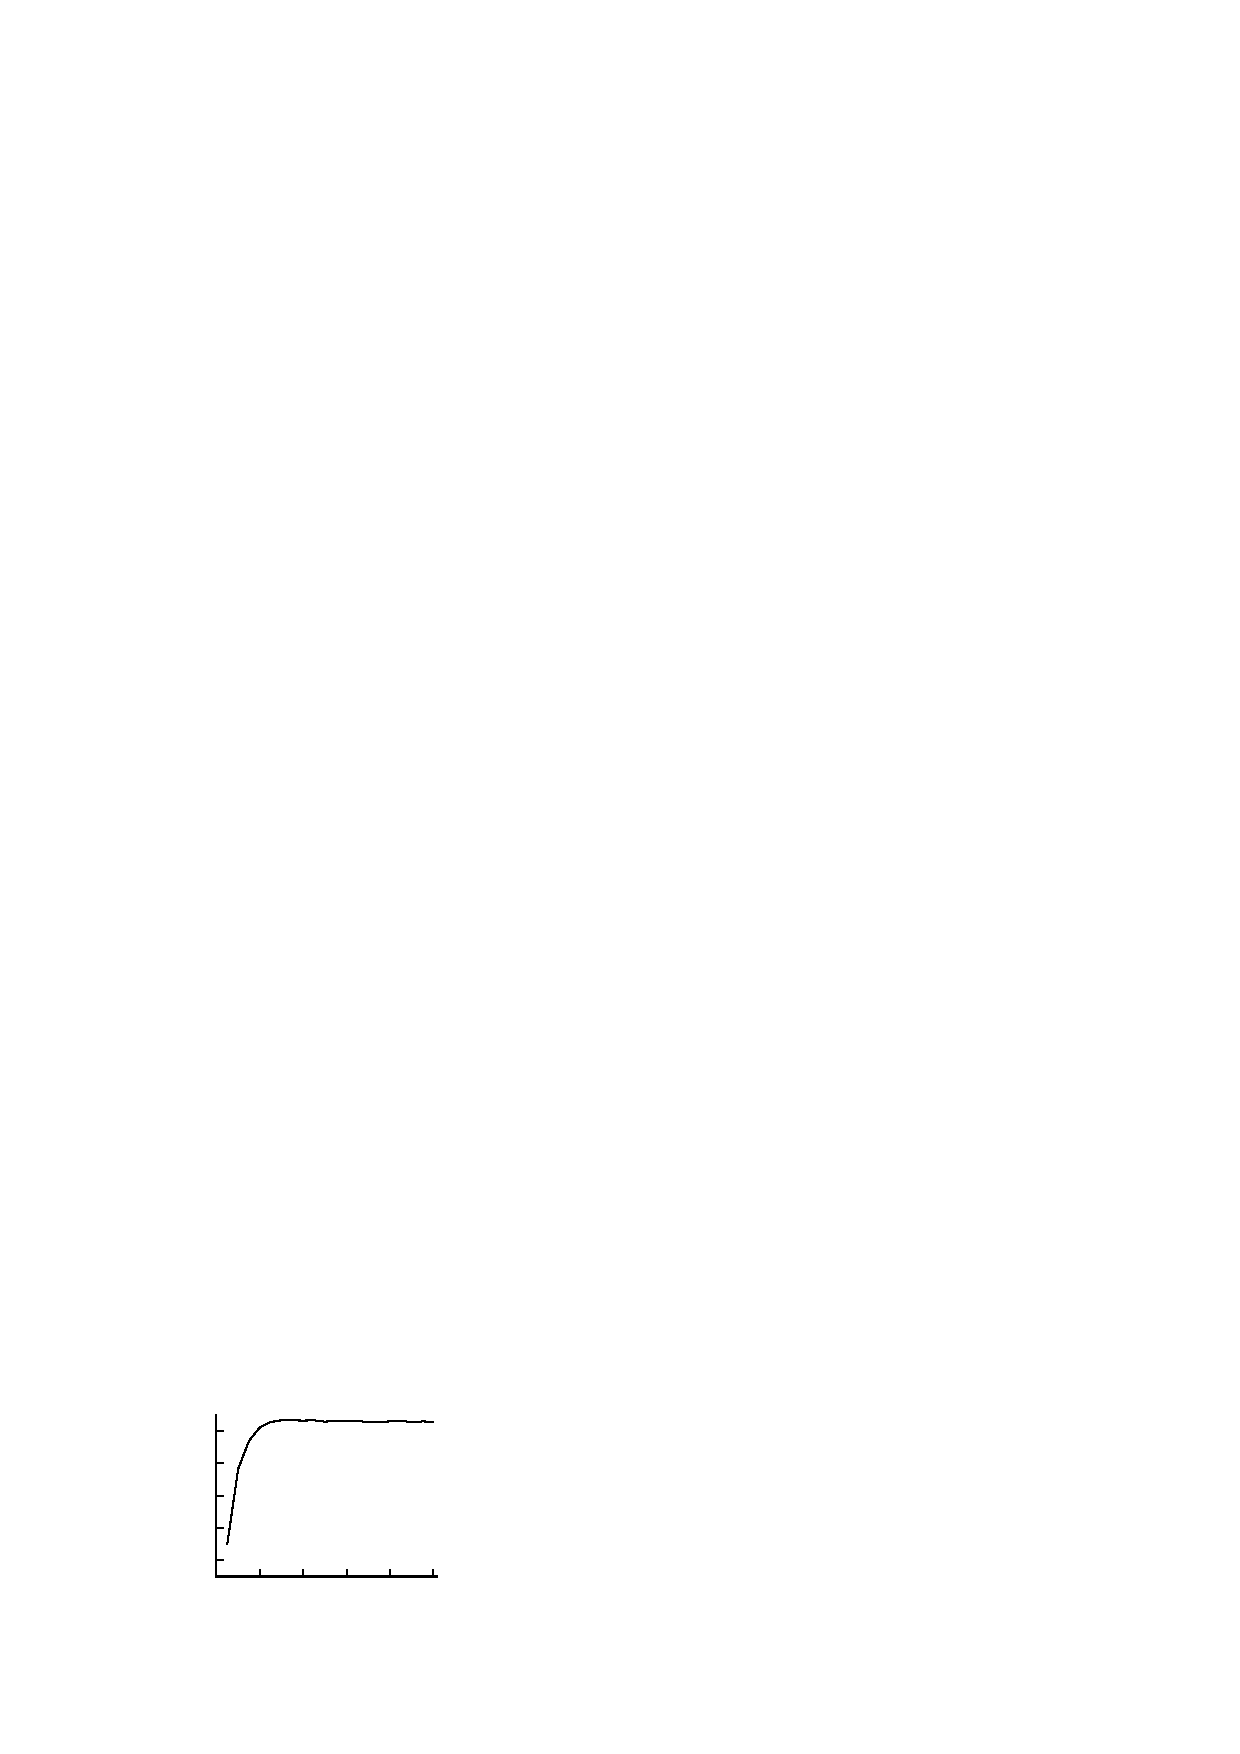
\includegraphics{fig_tau}}
    \put(0,0){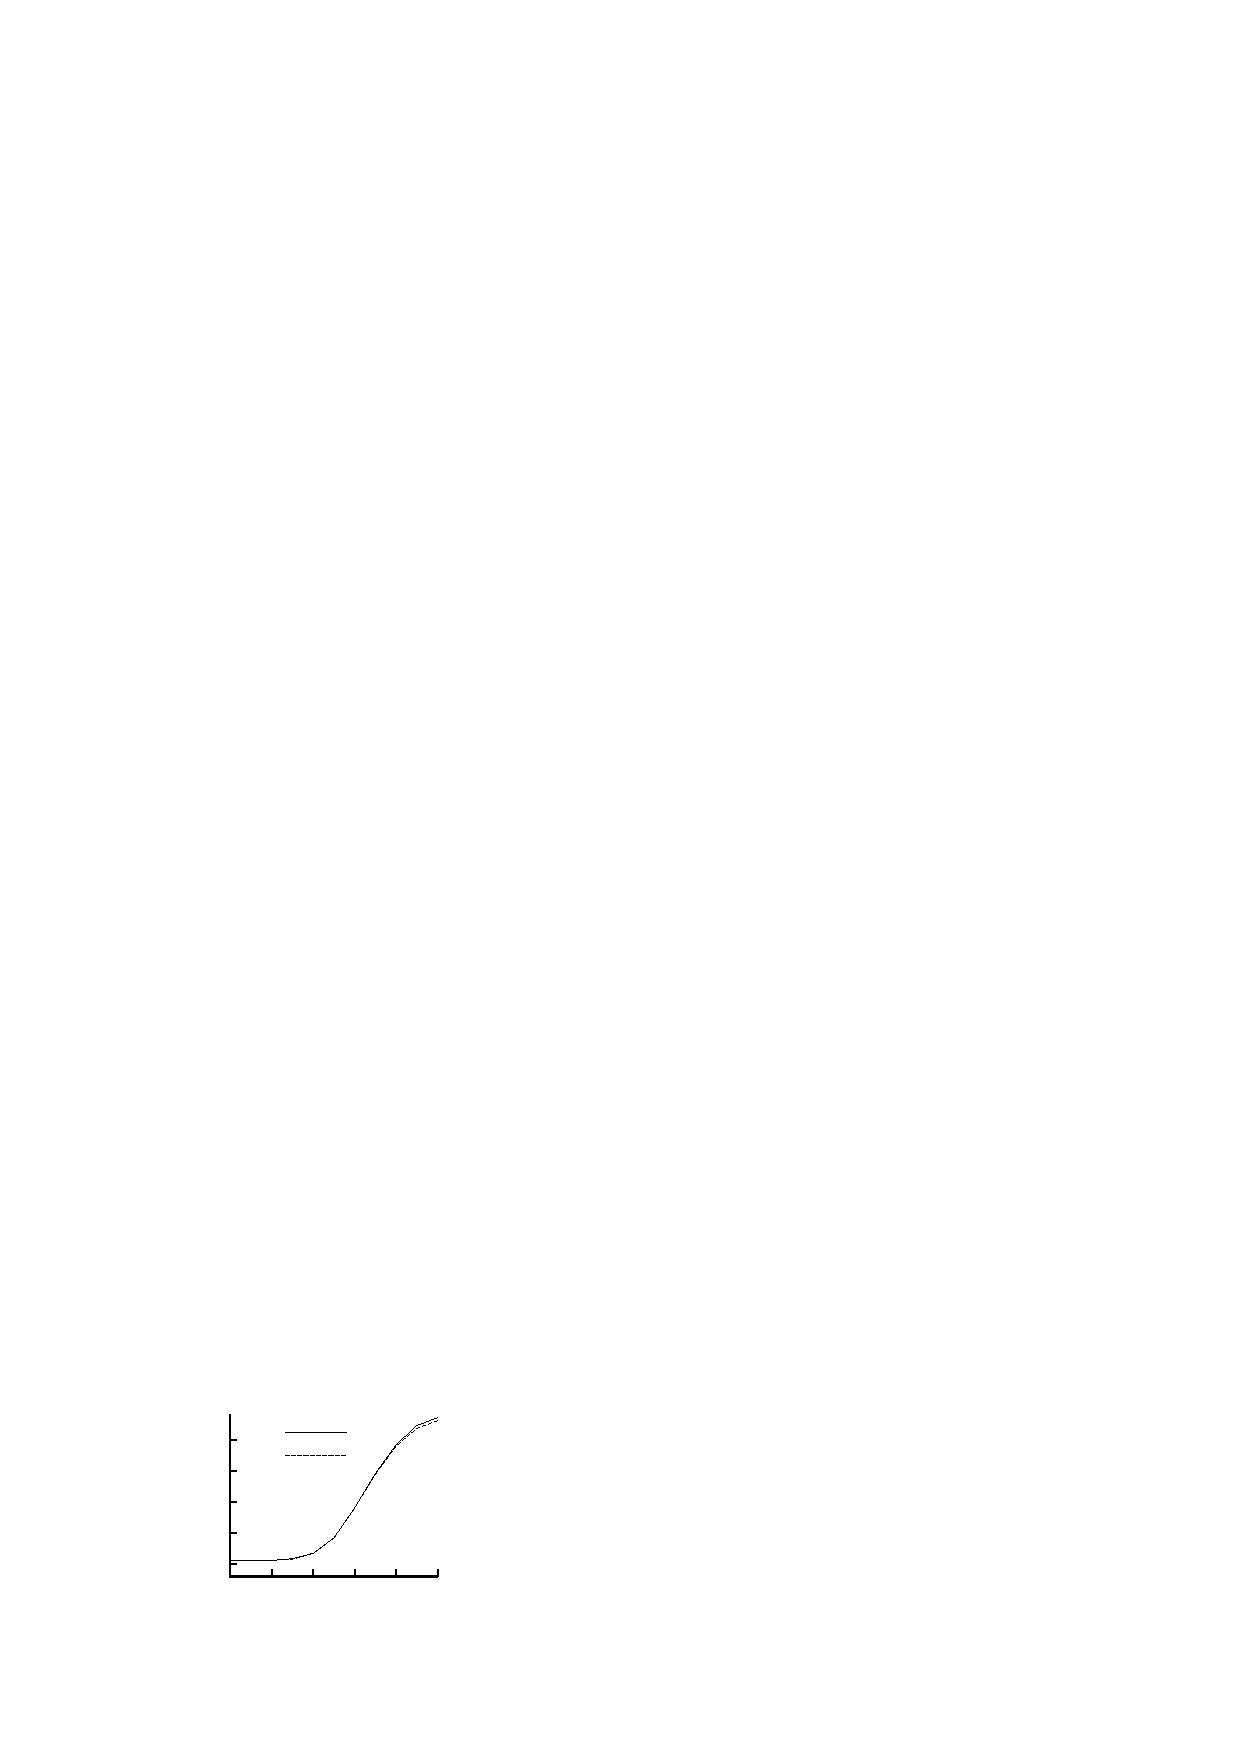
\includegraphics{fig_vp}}%


  \end{picture}%
\endgroup
\end{center}
\caption{The effect of the metric. In \textbf{A} the density
  estimation approach is applied using the Victor-Purpura metric
  instead of the van Rossum metric. This comparison uses the same
  simulated data as Fig.~\ref{fig_mu_sweep}, the estimated information
  using the van Rossum metric with $\tau=15\ms$ is marked
  \lq{}vr\rq{}. The Victor-Purpura metric has a \lq{}cost\rq{}
  parameter $q$, like $\tau$ in the van Rossum metric it expresses the
  precision of spike times in coding. Here $q=2/\tau$ and the
  corresponding estimate is marked \lq{}vp\rq{}. The two estimates are
  nearly identical.  In \textbf{B} the value of $\tau$ used in the
  metric in the density estimation approach is varied; generally the
  estimate does not depend sensitively on the value of $\tau$.
 \label{fig_metrics}}
\end{figure}


The sensitivity of the estimate to the choice of metric is examined in
Fig.~\ref{fig_metrics}. In Fig.~\ref{fig_metrics}\textbf{A} the van
Rossum metric is replaced by the Victor-Purpura metric
\citep{VictorPurpura1996}. This was the first metric proposed for
spike trains and rivals the van Rossum metric in measures of how well
metric distances capture information coding in spike trains
\citep{HoughtonVictor2010}. Furthermore, it is a non-Euclidean metric
\citep{AronovVictor2004}; the van Rossum metric works by embedding the
space of spike trains into the infinite-dimensional space of
functions, in this sense the van Rossum metric is Euclidean, replacing
it with the Victor Purpura metric demonstrates that this Euclidean
property is not required for the density estimation approach to
work. In Fig.~\ref{fig_metrics}\textbf{B} small values of $\tau$ show
a poor performance; for small values of $\tau$ the metric distance
between two spike trains is very dependent on noise which jitters
spike times to a degree that is significant when compared to $\tau$;
for values of $\tau$ that are similar or larger than the size of the
interval, the relative distances between different pairs of spike
train does not change as $\tau$ varies. The behaviour of the smoothing
parameter is explored in Fig.~\ref{fig_h}; Fig.~\ref{fig_h}\textbf{A}
shows an example of how the estimated mutual information depends on
$h$ and Fig.~\ref{fig_h}\textbf{B} graphs the change in the optimal
value of $h$ as the length of the spike trains changes.



\begin{figure}[tp]
\begin{center}
% GNUPLOT: LaTeX picture with Postscript
\begingroup
  \makeatletter
  \providecommand\color[2][]{%
    \GenericError{(gnuplot) \space\space\space\@spaces}{%
      Package color not loaded in conjunction with
      terminal option `colourtext'%
    }{See the gnuplot documentation for explanation.%
    }{Either use 'blacktext' in gnuplot or load the package
      color.sty in LaTeX.}%
    \renewcommand\color[2][]{}%
  }%
  \providecommand\includegraphics[2][]{%
    \GenericError{(gnuplot) \space\space\space\@spaces}{%
      Package graphicx or graphics not loaded%
    }{See the gnuplot documentation for explanation.%
    }{The gnuplot epslatex terminal needs graphicx.sty or graphics.sty.}%
    \renewcommand\includegraphics[2][]{}%
  }%
  \providecommand\rotatebox[2]{#2}%
  \@ifundefined{ifGPcolor}{%
    \newif\ifGPcolor
    \GPcolorfalse
  }{}%
  \@ifundefined{ifGPblacktext}{%
    \newif\ifGPblacktext
    \GPblacktexttrue
  }{}%
  % define a \g@addto@macro without @ in the name:
  \let\gplgaddtomacro\g@addto@macro
  % define empty templates for all commands taking text:
  \gdef\gplbacktext{}%
  \gdef\gplfronttext{}%
  \makeatother
  \ifGPblacktext
    % no textcolor at all
    \def\colorrgb#1{}%
    \def\colorgray#1{}%
  \else
    % gray or color?
    \ifGPcolor
      \def\colorrgb#1{\color[rgb]{#1}}%
      \def\colorgray#1{\color[gray]{#1}}%
      \expandafter\def\csname LTw\endcsname{\color{white}}%
      \expandafter\def\csname LTb\endcsname{\color{black}}%
      \expandafter\def\csname LTa\endcsname{\color{black}}%
      \expandafter\def\csname LT0\endcsname{\color[rgb]{1,0,0}}%
      \expandafter\def\csname LT1\endcsname{\color[rgb]{0,1,0}}%
      \expandafter\def\csname LT2\endcsname{\color[rgb]{0,0,1}}%
      \expandafter\def\csname LT3\endcsname{\color[rgb]{1,0,1}}%
      \expandafter\def\csname LT4\endcsname{\color[rgb]{0,1,1}}%
      \expandafter\def\csname LT5\endcsname{\color[rgb]{1,1,0}}%
      \expandafter\def\csname LT6\endcsname{\color[rgb]{0,0,0}}%
      \expandafter\def\csname LT7\endcsname{\color[rgb]{1,0.3,0}}%
      \expandafter\def\csname LT8\endcsname{\color[rgb]{0.5,0.5,0.5}}%
    \else
      % gray
      \def\colorrgb#1{\color{black}}%
      \def\colorgray#1{\color[gray]{#1}}%
      \expandafter\def\csname LTw\endcsname{\color{white}}%
      \expandafter\def\csname LTb\endcsname{\color{black}}%
      \expandafter\def\csname LTa\endcsname{\color{black}}%
      \expandafter\def\csname LT0\endcsname{\color{black}}%
      \expandafter\def\csname LT1\endcsname{\color{black}}%
      \expandafter\def\csname LT2\endcsname{\color{black}}%
      \expandafter\def\csname LT3\endcsname{\color{black}}%
      \expandafter\def\csname LT4\endcsname{\color{black}}%
      \expandafter\def\csname LT5\endcsname{\color{black}}%
      \expandafter\def\csname LT6\endcsname{\color{black}}%
      \expandafter\def\csname LT7\endcsname{\color{black}}%
      \expandafter\def\csname LT8\endcsname{\color{black}}%
    \fi
  \fi
  \setlength{\unitlength}{0.0500bp}%
  \begin{picture}(7300.00,2520.00)%


      \put(846,2700){\makebox(0,0)[r]{\strut{} \textbf{A}}}%


      \put(946,704){\makebox(0,0)[r]{\strut{} 0}}%
      \put(946,1092){\makebox(0,0)[r]{\strut{} 0.2}}%
      \put(946,1480){\makebox(0,0)[r]{\strut{} 0.4}}%
      \put(946,1868){\makebox(0,0)[r]{\strut{} 0.6}}%
      \put(946,2256){\makebox(0,0)[r]{\strut{} 0.8}}%
      \put(1582,484){\makebox(0,0){\strut{} 150}}%
      \put(2122,484){\makebox(0,0){\strut{} 300}}%
      \put(2663,484){\makebox(0,0){\strut{} 450}}%
      \put(3203,484){\makebox(0,0){\strut{} 600}}%
      \put(176,1480){\rotatebox{-270}{\makebox(0,0){\strut{}mutual information (bits)}}}%
      \put(2140,154){\makebox(0,0){\strut{}$h$}}%


      \put(4546,2700){\makebox(0,0)[r]{\strut{} \textbf{B}}}%

      \put(4646,704){\makebox(0,0)[r]{\strut{} 0}}%
      \put(4646,1014){\makebox(0,0)[r]{\strut{} 50}}%
      \put(4646,1325){\makebox(0,0)[r]{\strut{} 100}}%
      \put(4646,1635){\makebox(0,0)[r]{\strut{} 150}}%
      \put(4646,1946){\makebox(0,0)[r]{\strut{} 200}}%
      \put(4646,2256){\makebox(0,0)[r]{\strut{} 250}}%
      \put(5289,484){\makebox(0,0){\strut{} 100}}%
      \put(5827,484){\makebox(0,0){\strut{} 200}}%
      \put(6365,484){\makebox(0,0){\strut{} 300}}%
      \put(6903,484){\makebox(0,0){\strut{} 400}}%
      \put(3876,1480){\rotatebox{-270}{\makebox(0,0){\strut{}$h$}}}%
      \put(5840,154){\makebox(0,0){\strut{}spike train length (s)}}%

    \put(3700,0){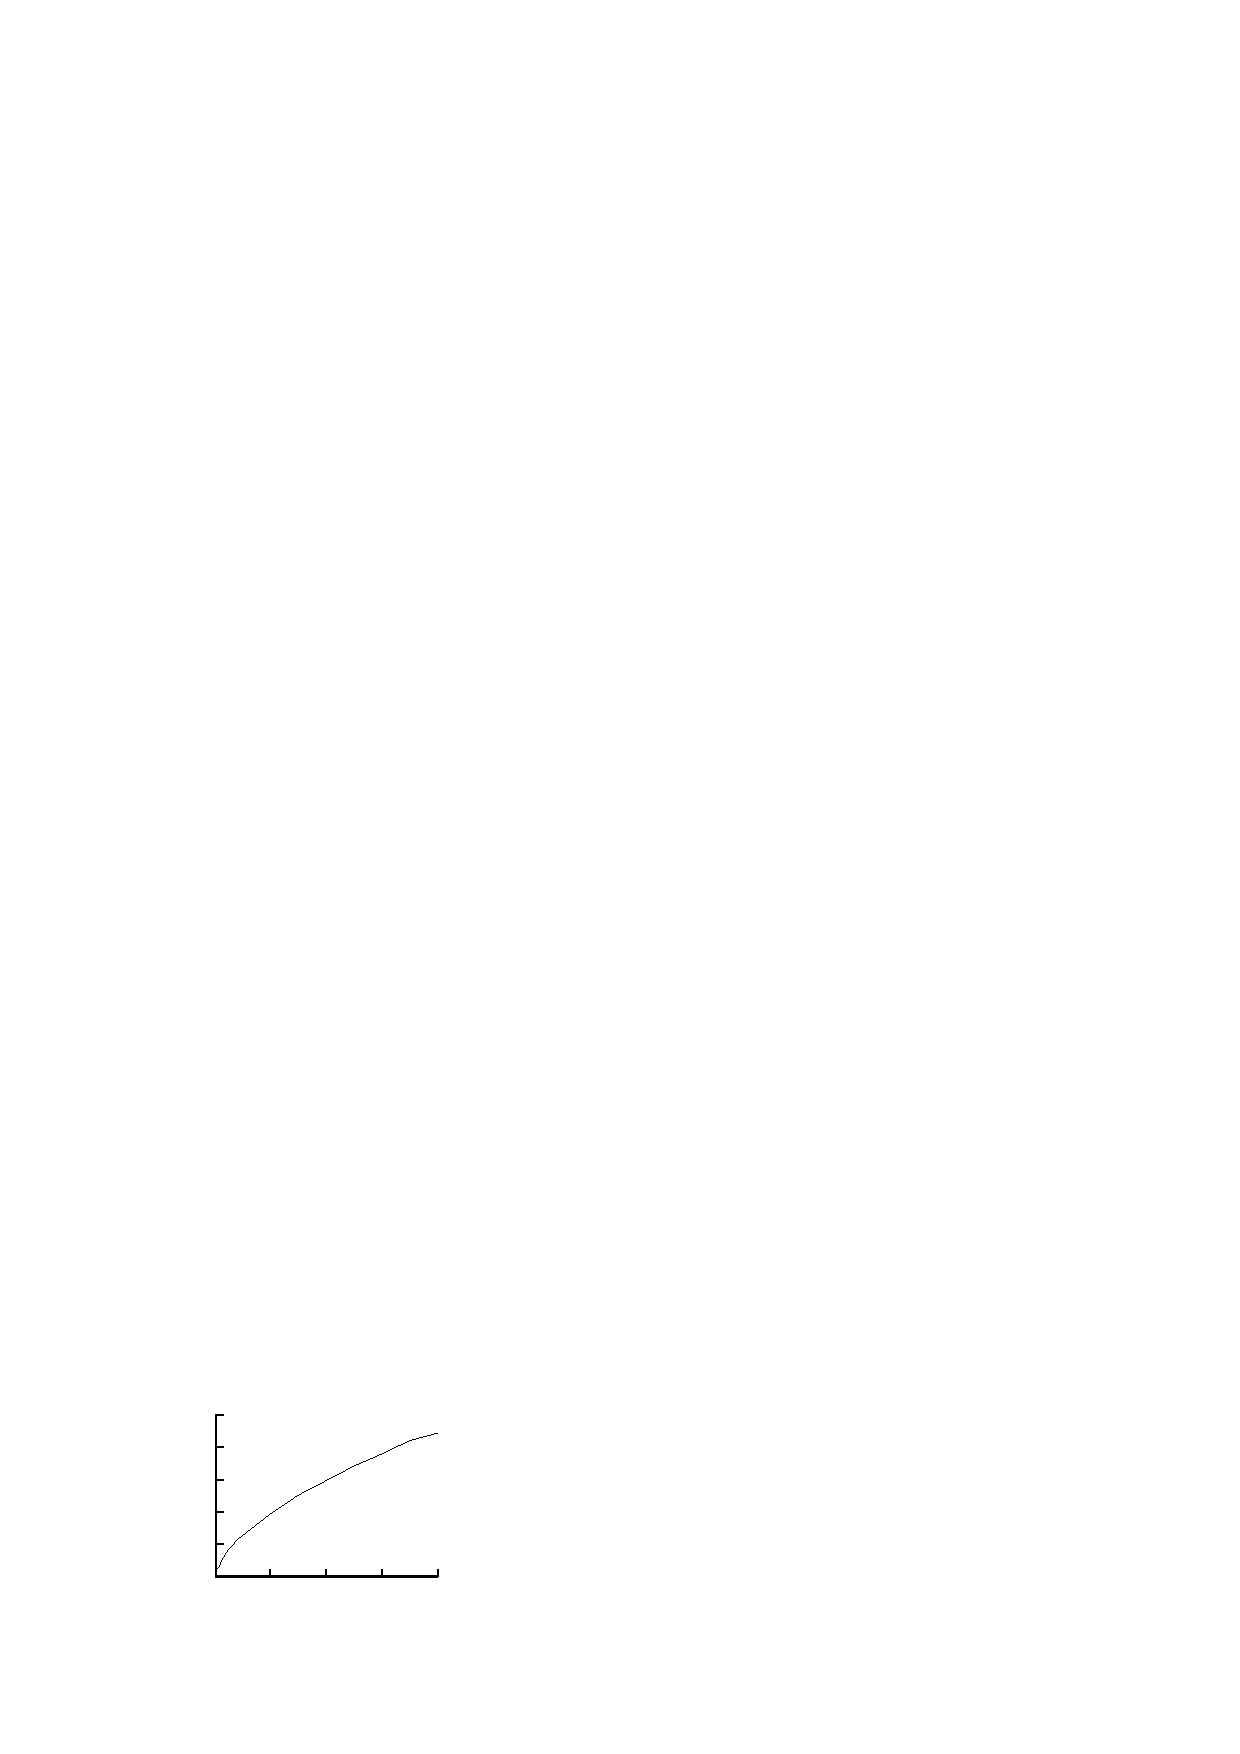
\includegraphics{fig_best_h}}
    \put(0,0){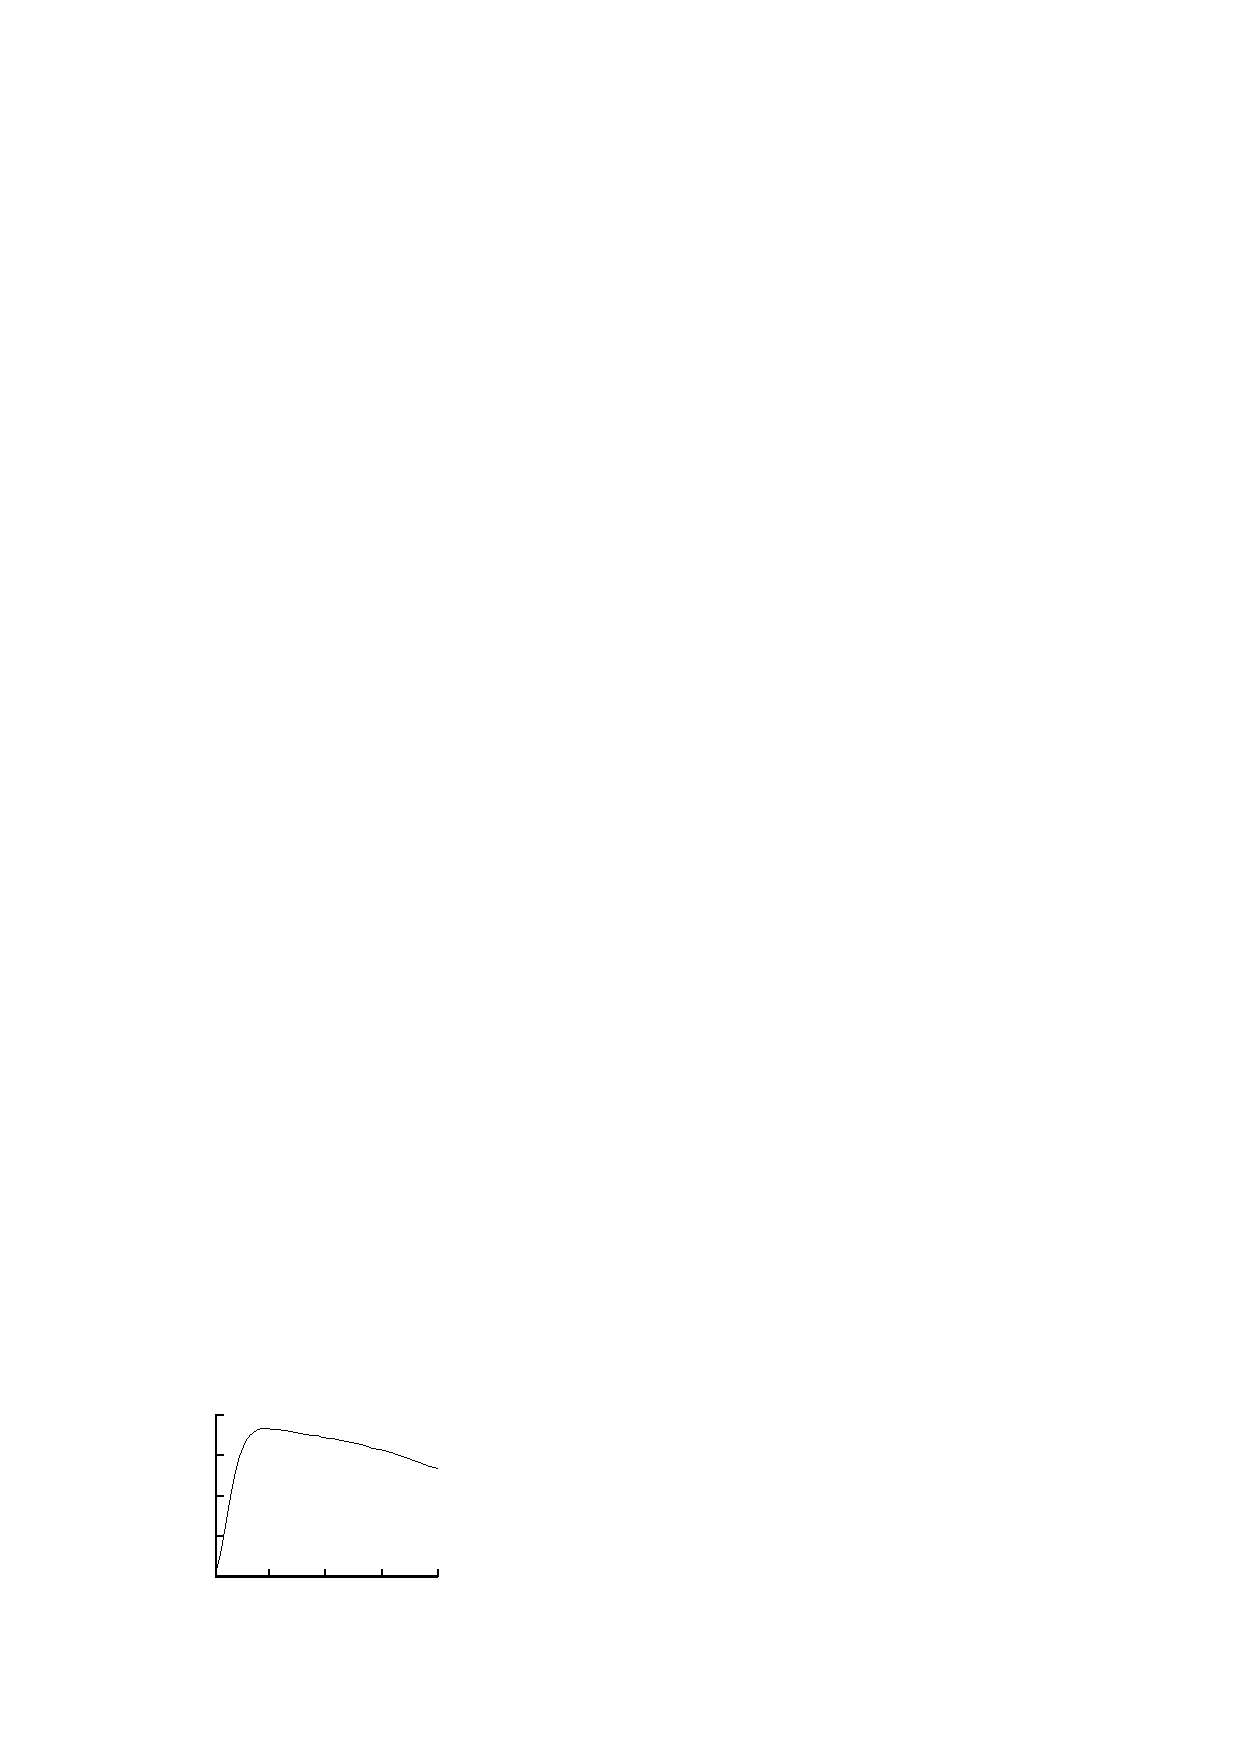
\includegraphics{fig_h_sweep}}%

  \end{picture}%
\endgroup
\end{center}
\caption{The smoothing parameter $h$. In both these graphs the mutual
  information is estimated for $\mu=0.7$. In \textbf{A} the estimated
  mutual information is plotted against $h$ using 200 s of spike
  train.  In \textbf{B} the optimal value of $h$, that is the $h$
  maximizing the estimated information, is plotted as a function of
  the spike train length.
 \label{fig_h}}
\end{figure}



\section{Discussion}

This paper describes a method for choosing the smoothing parameter for
a Kozachenko-Leonenko estimator of the mutual information and tests it
on fictive spike train data. It is seen that the density estimation
method is very effective in estimating the mutual information using
much smaller amounts of data than that required for the
discretization-based approach. 

It is hoped that this approach will prove useful in estimating mutual
information for real data. Obviously using the approach in practice
will require a choice of the interval length and of spike train
metric. Typically, as with the binned approach, the interval length
should be chosen to reflect the time scale of interest for the cells
being studied, this might, for example, reflect the membrane constants
of the cells and the correlation length of their stimuli. Hopefully
the density estimation method will allow longer interval lengths to be
used than was possible with the binned approach. If the van Rossum
metric is used, the parameter $\tau$ needs to be set; ideally this
value should maximize the estimated mutual information, often
$\tau=15\ms$ is used for van Rossum metrics. There are also measures
of spike train similarity \cite{KreuzEtAl2007,KreuzEtAl2012} that
adapt to the time-local spike rate and do not have a parameter like
the $\tau$ in the van Rossum metric, or the $q$ in the Victor-Purpura
metric; these would avoid the need to fix the metric parameters.

The density estimation approach is more computationally demanding than
the binned approach; the whole matrix of distances between pairs of
interval pairs must be calculated and for each interval pair the
nearest $h$ other pairs needs to be found.

In the density estimation method, the information is estimated from
the matrix of distance values. This means that any
information-carrying features of the spike trains that are not
captured by the metric will be lost in the estimate of mutual
information. Spike train metrics are often evaluated using transmitted
information \citep{VictorPurpura1996,HoughtonVictor2010}, they are, in
this sense, designed to capture the information-carrying
features. However, mutual information estimated from a distance matrix
must underestimate the true value. In the example considered here,
this underestimate appears to be small; there may be some indication
that the underestimate increases as the number of spikes
increases. This might be a more significant for real data where there
may be information-carry motifs in spike trains, there are none in
the simulated data. 

The Kozachenko-Leonenko estimator is a powerful approach to
calculating mutual information based on the proximity structure of the
data; it is often more efficient than estimators that do not
incorporate this structure. It has also been shown in
\citet{Houghton2015} that is does not require that there are useful
co\"{o}rdinates for the spaces the random variables take their values
on.  Obviously this is the case when the data of interest is spike
train data, but there are likely to be manifold other applications to
other data types, including other applications involving neuroscience
data, such as calculating the mutual information between spiking
responses and a continuous stimulus space, as previously considered in
\cite{PanzeriEtAl1999}.


\subsection*{Acknowledgements} Thanks to the  James S. McDonnell Foundation for support through a  Scholar Award in Cognition (JSMF \#220020239; https://www.jsmf.org/). This work was carried out using the computational facilities of the Advanced Computing Research Centre, University of Bristol - http://www.bris.ac.uk/acrc/.


\begin{thebibliography}{}

\bibitem[\protect\astroncite{Aronov et~al.}{2003}]{AronovEtAl2003}
Aronov, D., Reich, D.~S., Mechler, F., and Victor, J.~D. (2003).
\newblock Neural coding of spatial phase in v1 of the macaque monkey.
\newblock {\em Journal of Neurophysiology}, 89(6):3304--3327.

\bibitem[\protect\astroncite{Aronov and Victor}{2004}]{AronovVictor2004}
Aronov, D. and Victor, J.~D. (2004).
\newblock Non-euclidean properties of spike train metric spaces.
\newblock {\em Physical Review E}, 69(6):061905.

\bibitem[\protect\astroncite{Houghton}{2015}]{Houghton2015}
Houghton, C. (2015).
\newblock Calculating mutual information for spike trains and other data with
  distances but no coordinates.
\newblock {\em Royal Society Open Science}, 2(5):140391.

\bibitem[\protect\astroncite{Houghton and Kreuz}{2012}]{HoughtonKreuz2012}
Houghton, C. and Kreuz, T. (2012).
\newblock On the efficient calculation of van rossum distances.
\newblock {\em Network: Computation in Neural Systems}, 23(1-2):48--58.

\bibitem[\protect\astroncite{Houghton and Sen}{2008}]{HoughtonSen2008}
Houghton, C. and Sen, K. (2008).
\newblock A new multineuron spike train metric.
\newblock {\em Neural Computation}, 20(6):1495--1511.

\bibitem[\protect\astroncite{Houghton and Victor}{2010}]{HoughtonVictor2010}
Houghton, C. and Victor, J. (2010).
\newblock Measuring representational distances--the spike-train metrics
  approach.
\newblock {\em Visual Population Codes--Toward a Common Multivariate Framework
  for Cell Recording and Functional Imaging}, pages 391--416.

\bibitem[\protect\astroncite{Kiefer}{1953}]{Kiefer1953}
Kiefer, J. (1953).
\newblock Sequential minimax search for a maximum.
\newblock {\em Proceedings of the American Mathematical Society},
  4(3):502--506.

\bibitem[\protect\astroncite{Kozachenko and
  Leonenko}{1987}]{KozachenkoLeonenko1987}
Kozachenko, L. and Leonenko, N.~N. (1987).
\newblock Sample estimate of the entropy of a random vector.
\newblock {\em Problemy Peredachi Informatsii}, 23(2):9--16.

\bibitem[\protect\astroncite{Kraskov et~al.}{2004}]{KraskovEtAl2004}
Kraskov, A., St{\"o}gbauer, H., and Grassberger, P. (2004).
\newblock Estimating mutual information.
\newblock {\em Physical Review E}, 69(6):066138.

\bibitem[\protect\astroncite{Kreuz et~al.}{2012}]{KreuzEtAl2012}
Kreuz, T., Chicharro, D., Houghton, C., Andrzejak, R.~G., and Mormann, F.
  (2012).
\newblock Monitoring spike train synchrony.
\newblock {\em Journal of Neurophysiology}, 109(5):1457--1472.

\bibitem[\protect\astroncite{Kreuz et~al.}{2007}]{KreuzEtAl2007}
Kreuz, T., Haas, J.~S., Morelli, A., Abarbanel, H.~D., and Politi, A. (2007).
\newblock Measuring spike train synchrony.
\newblock {\em Journal of neuroscience methods}, 165(1):151--161.

\bibitem[\protect\astroncite{Magri et~al.}{2009}]{MagriEtAl2009}
Magri, C., Whittingstall, K., Singh, V., Logothetis, N.~K., and Panzeri, S.
  (2009).
\newblock A toolbox for the fast information analysis of multiple-site {LFP},
  {EEG} and spike train recordings.
\newblock {\em BMC Neuroscience}, 10(1):81.

\bibitem[\protect\astroncite{Montemurro et~al.}{2007}]{MontemurroEtAl2007}
Montemurro, M.~A., Senatore, R., and Panzeri, S. (2007).
\newblock Tight data-robust bounds to mutual information combining shuffling
  and model selection techniques.
\newblock {\em Neural Computation}, 19(11):2913--2957.

\bibitem[\protect\astroncite{Nemenman et~al.}{2004}]{NemenmanEtAl2004}
Nemenman, I., Bialek, W., and van Steveninck, R. d.~R. (2004).
\newblock Entropy and information in neural spike trains: Progress on the
  sampling problem.
\newblock {\em Physical Review E}, 69(5):056111.

\bibitem[\protect\astroncite{Nirenberg et~al.}{2001}]{NirenbergEtAl2001}
Nirenberg, S., Carcieri, S.~M., Jacobs, A.~L., and Latham, P.~E. (2001).
\newblock Retinal ganglion cells act largely as independent encoders.
\newblock {\em Nature}, 411(6838):698.

\bibitem[\protect\astroncite{Panzeri et~al.}{2007}]{PanzeriEtAl2007}
Panzeri, S., Senatore, R., Montemurro, M.~A., and Petersen, R.~S. (2007).
\newblock Correcting for the sampling bias problem in spike train information
  measures.
\newblock {\em Journal of Neurophysiology}, 98(3):1064--1072.

\bibitem[\protect\astroncite{Panzeri et~al.}{1999}]{PanzeriEtAl1999}
Panzeri, S., Treves, A., Schultz, S., and Rolls, E.~T. (1999).
\newblock On decoding the responses of a population of neurons from short time
  windows.
\newblock {\em Neural Computation}, 11(7):1553--1577.

\bibitem[\protect\astroncite{Rossum}{2001}]{vanRossum2001}
Rossum, M.~v. (2001).
\newblock A novel spike distance.
\newblock {\em Neural Computation}, 13(4):751--763.

\bibitem[\protect\astroncite{Strong et~al.}{1998}]{StrongEtAl1998}
Strong, S.~P., Koberle, R., van Steveninck, R. R.~R., and Bialek, W. (1998).
\newblock Entropy and information in neural spike trains.
\newblock {\em Physical Review Letters}, 80(1):197.

\bibitem[\protect\astroncite{Tobin and Houghton}{2013}]{TobinHoughton2013}
Tobin, R.~J. and Houghton, C.~J. (2013).
\newblock A kernel-based calculation of information on a metric space.
\newblock {\em Entropy}, 15(10):4540--4552.

\bibitem[\protect\astroncite{Treves and Panzeri}{1995}]{TrevesPanzeri1995}
Treves, A. and Panzeri, S. (1995).
\newblock The upward bias in measures of information derived from limited data
  samples.
\newblock {\em Neural Computation}, 7(2):399--407.

\bibitem[\protect\astroncite{Victor}{2002}]{Victor2002}
Victor, J.~D. (2002).
\newblock Binless strategies for estimation of information from neural data.
\newblock {\em Physical Review E}, 66(5):051903.

\bibitem[\protect\astroncite{Victor and Purpura}{1996}]{VictorPurpura1996}
Victor, J.~D. and Purpura, K.~P. (1996).
\newblock Nature and precision of temporal coding in visual cortex: a
  metric-space analysis.
\newblock {\em Journal of Neurophysiology}, 76(2):1310--1326.

\end{thebibliography}

\end{document}


